\documentclass[hyperref=colorlinks]{beamer}
\mode<presentation>
\usetheme{iclpt}
\setbeamertemplate{navigation symbols}{}
\setbeamertemplate{headline}{
  \begin{beamercolorbox}[leftskip=.2cm,rightskip=.2cm,topskip=.2cm,ht=1.1cm,dp=0.1cm,wd=\textwidth]{institute in head/foot}
    
\includegraphics[height=1cm]{icl.pdf}
    \hfill
    
\includegraphics[height=1cm]{../Pics/CMS-Color.pdf}
  \end{beamercolorbox}
}
\setbeamertemplate{footline}{
  \begin{beamercolorbox}[ht=.35cm,dp=0.2cm,wd=\textwidth,leftskip=.3cm]{author in head/foot}%
    \begin{minipage}[c]{5cm}%
      \usebeamerfont{author in head/foot}
      \insertshortauthor 
      \insertshorttitle
    \end{minipage}\hfill%
    \hfill
    \insertframenumber{} / \pageref{lastframe}
    %\hfill
    \begin{minipage}{6cm}
      \hfill
      %\insertshorttitle
    \end{minipage}
  \end{beamercolorbox}%
}

\usepackage{color}
\usepackage{tabularx,colortbl}
\usepackage{graphicx}
\usepackage{pdfpages}
\usepackage{feynmp}
\usepackage{rotating}
\usepackage{moresize}
\usepackage{xcolor,colortbl}
\DeclareGraphicsRule{*}{mps}{*}{}

\title[Invisible Higgs at CMS]{\vspace{-0.2cm} Searches for invisible decay modes of the Higgs boson with the CMS detector}
\author[P. Dunne]{\underline{P. Dunne} - Imperial College London \\ on behalf of the CMS Collaboration \\ PANIC 2014 - 26/08/2014} % A.M. Magnan and A. Nikitenko Joao Pela with \\ R. Aggleton, J. Brooke: Bristol \\ C.Asawangtrakuldee, Q.Li: Peking \\ P. Srimanobhas: Chulalongkorn \\ S. Kumar, K. Mazumdar: Mumbai}
\titlegraphic{
  \vspace{-0.7cm}
  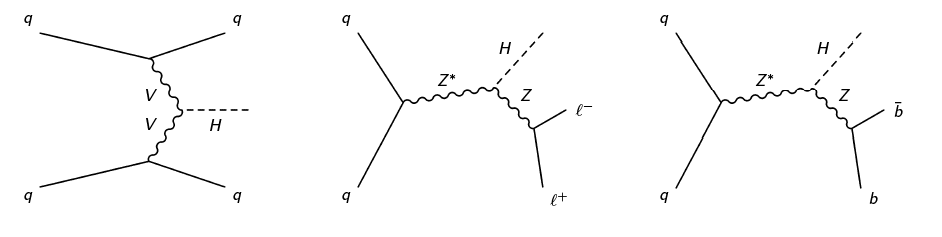
\includegraphics[width=\textwidth]{TalkPics/invcomb021213/feyndiags}
  %% \begin{fmfgraph*}(100,70)
  %%         \fmfleft{i1,i2}
  %%         \fmfright{o1,o2,o3}
  %%         \fmf{fermion}{i1,v1,o1}
  %%         \fmf{fermion}{i2,v2,o3}
  %%         \fmf{phantom,tension=4/5}{v1,v2}
  %%         \fmffreeze
  %%         \fmf{photon,label=$W,,Z$}{v1,v3}
  %%         \fmf{photon,label=$W,,Z$}{v2,v3}
  %%         \fmf{dashes}{v3,o2}
  %%         \fmflabel{$q$}{i1}
  %%         \fmflabel{$q$}{i2}
  %%         \fmflabel{$q$}{o1}
  %%         \fmflabel{$q$}{o3}
  %%         \fmflabel{$H$}{o2}

  %%       \end{fmfgraph*}
}
\date{}
\begin{document}
\begin{fmffile}{panicfeynmandiags}

  %TITLE PAGE
  \section{Title}
  \begin{frame}
    \titlepage
    
  \end{frame}

  \begin{frame}
    \frametitle{Why Higgs to Invisible?}
    \vspace{-.2cm}
    \begin{columns}
      \column{.5\textwidth}
      \begin{block}{\scriptsize Experimental motivation}
        \scriptsize
        \begin{itemize}
        \item Current measurements of the 125 GeV Higgs boson are compatible with Standard Model (SM) expectations
        \item[-] large uncertainties can still accommodate significant beyond the SM (BSM) properties
        \item Additional Higgs bosons with exotic decays are not excluded
        \end{itemize}
      \end{block}
      \column{.45\textwidth}
      \hfill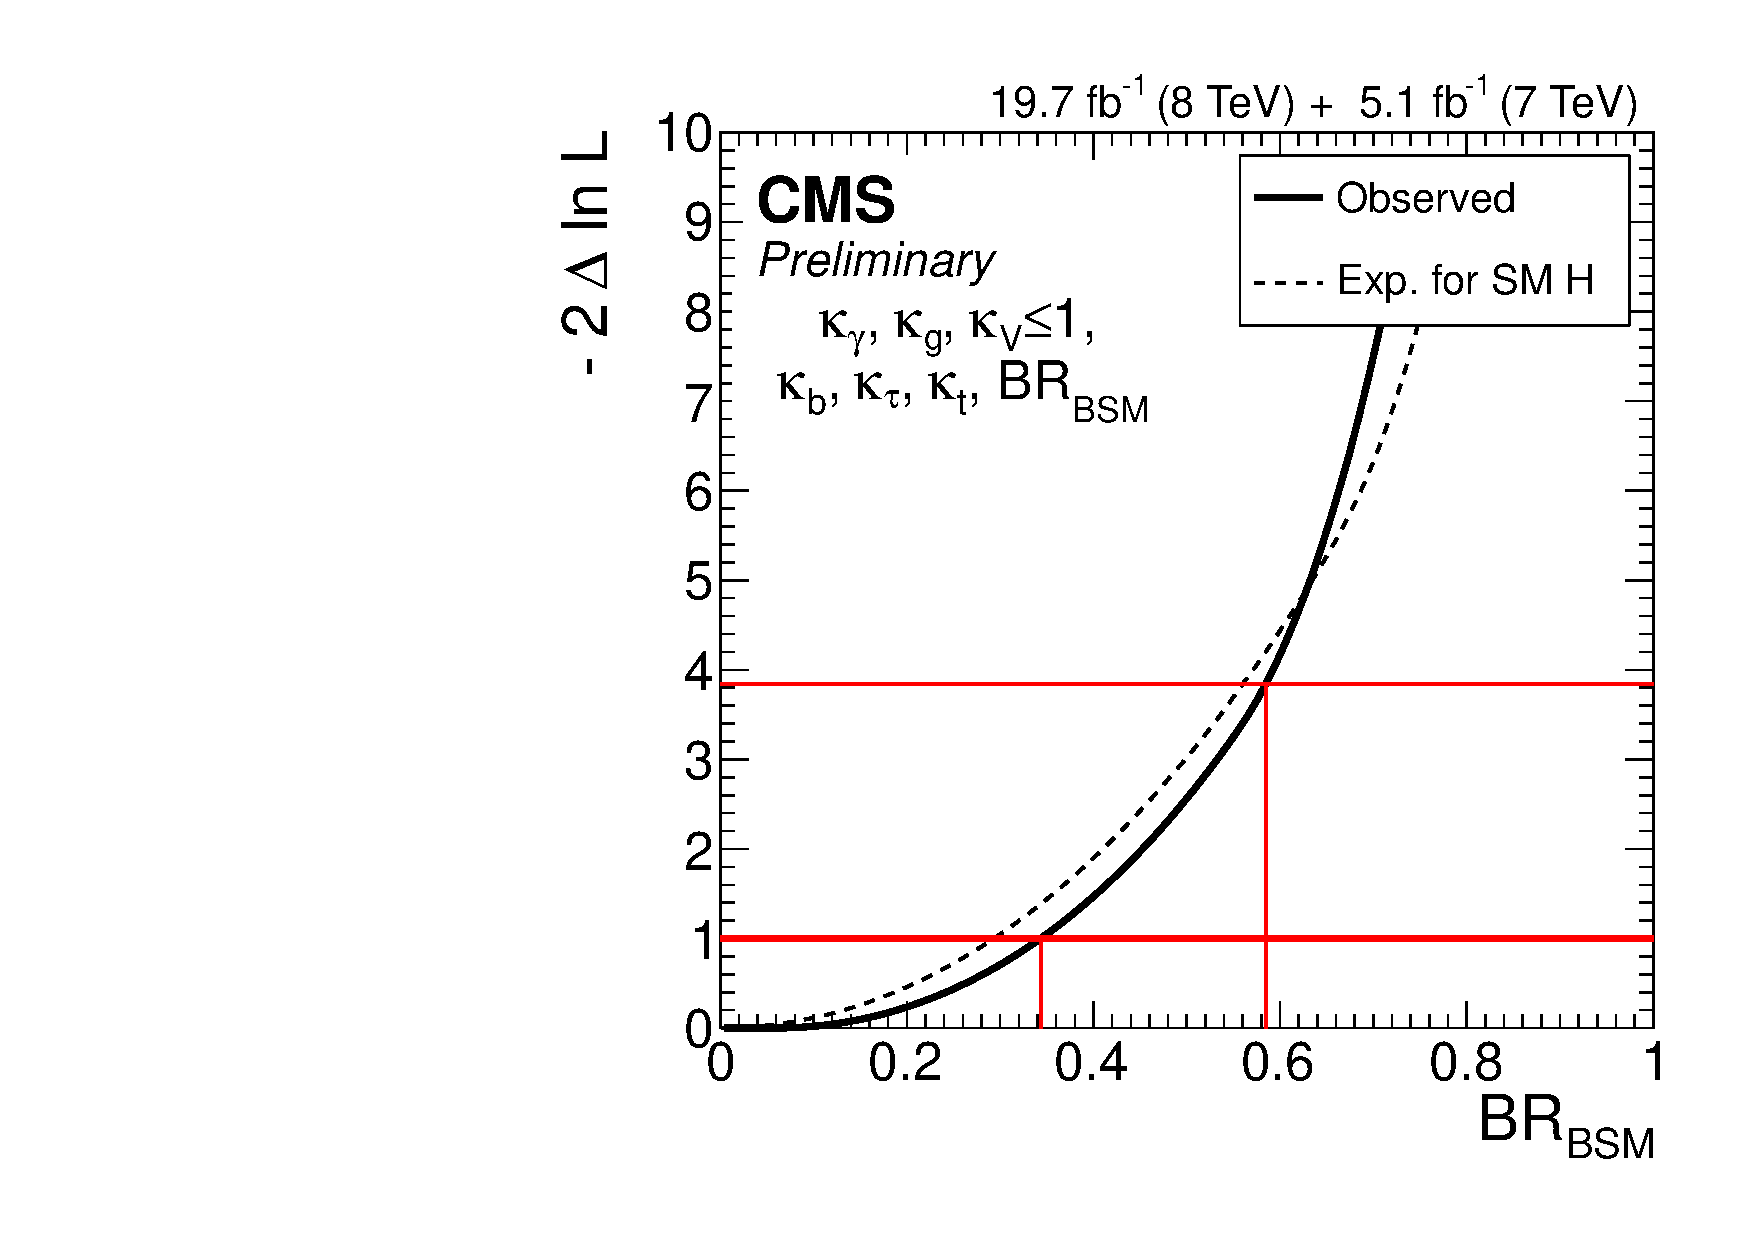
\includegraphics[height=.55\textheight]{TalkPics/panicpics/indirectbrbsm.pdf}
      \column{.05\textwidth}
      \begin{turn}{-90}\scriptsize CMS-PAS-HIG-14-009\end{turn}
    \end{columns}
    \begin{columns}
      \column{1.095\textwidth}
      \begin{block}{\scriptsize Theoretical motivation}
        \scriptsize
        \begin{itemize}
        \item Many BSM theories predict Higgs boson decays to invisible final states:
        \item[-] e.g. SUSY, extra dimensions, fourth-generation neutrinos
        \item These final state particles are often dark matter candidates
        \end{itemize}
      \end{block}
    \end{columns}

  \end{frame}

  \begin{frame}
    \frametitle{Direct and Indirect Searches}

    \begin{columns}
      \column{.5\textwidth}
      \vspace{-.8cm}
      \begin{block}{\scriptsize Indirect searches}
        \begin{itemize}
          \scriptsize
        \item BSM Higgs decays affect the total Higgs width:
        \item[-] $\Gamma_{tot} = \Gamma^{SM}_{tot}\cdot\frac{\sum\limits^{obs}_{x}\kappa_{x}^{2}\cdot BR_{x}^{SM}}{1-BR_{BSM}}, \kappa_{x}^{2}=\frac{\Gamma^{obs}_{x}}{\Gamma^{SM}_{x}}$
        \item Visible decays can, therefore, constrain the invisible branching fraction
        \end{itemize}
      \end{block}
      \column{.45\textwidth}

      \hfill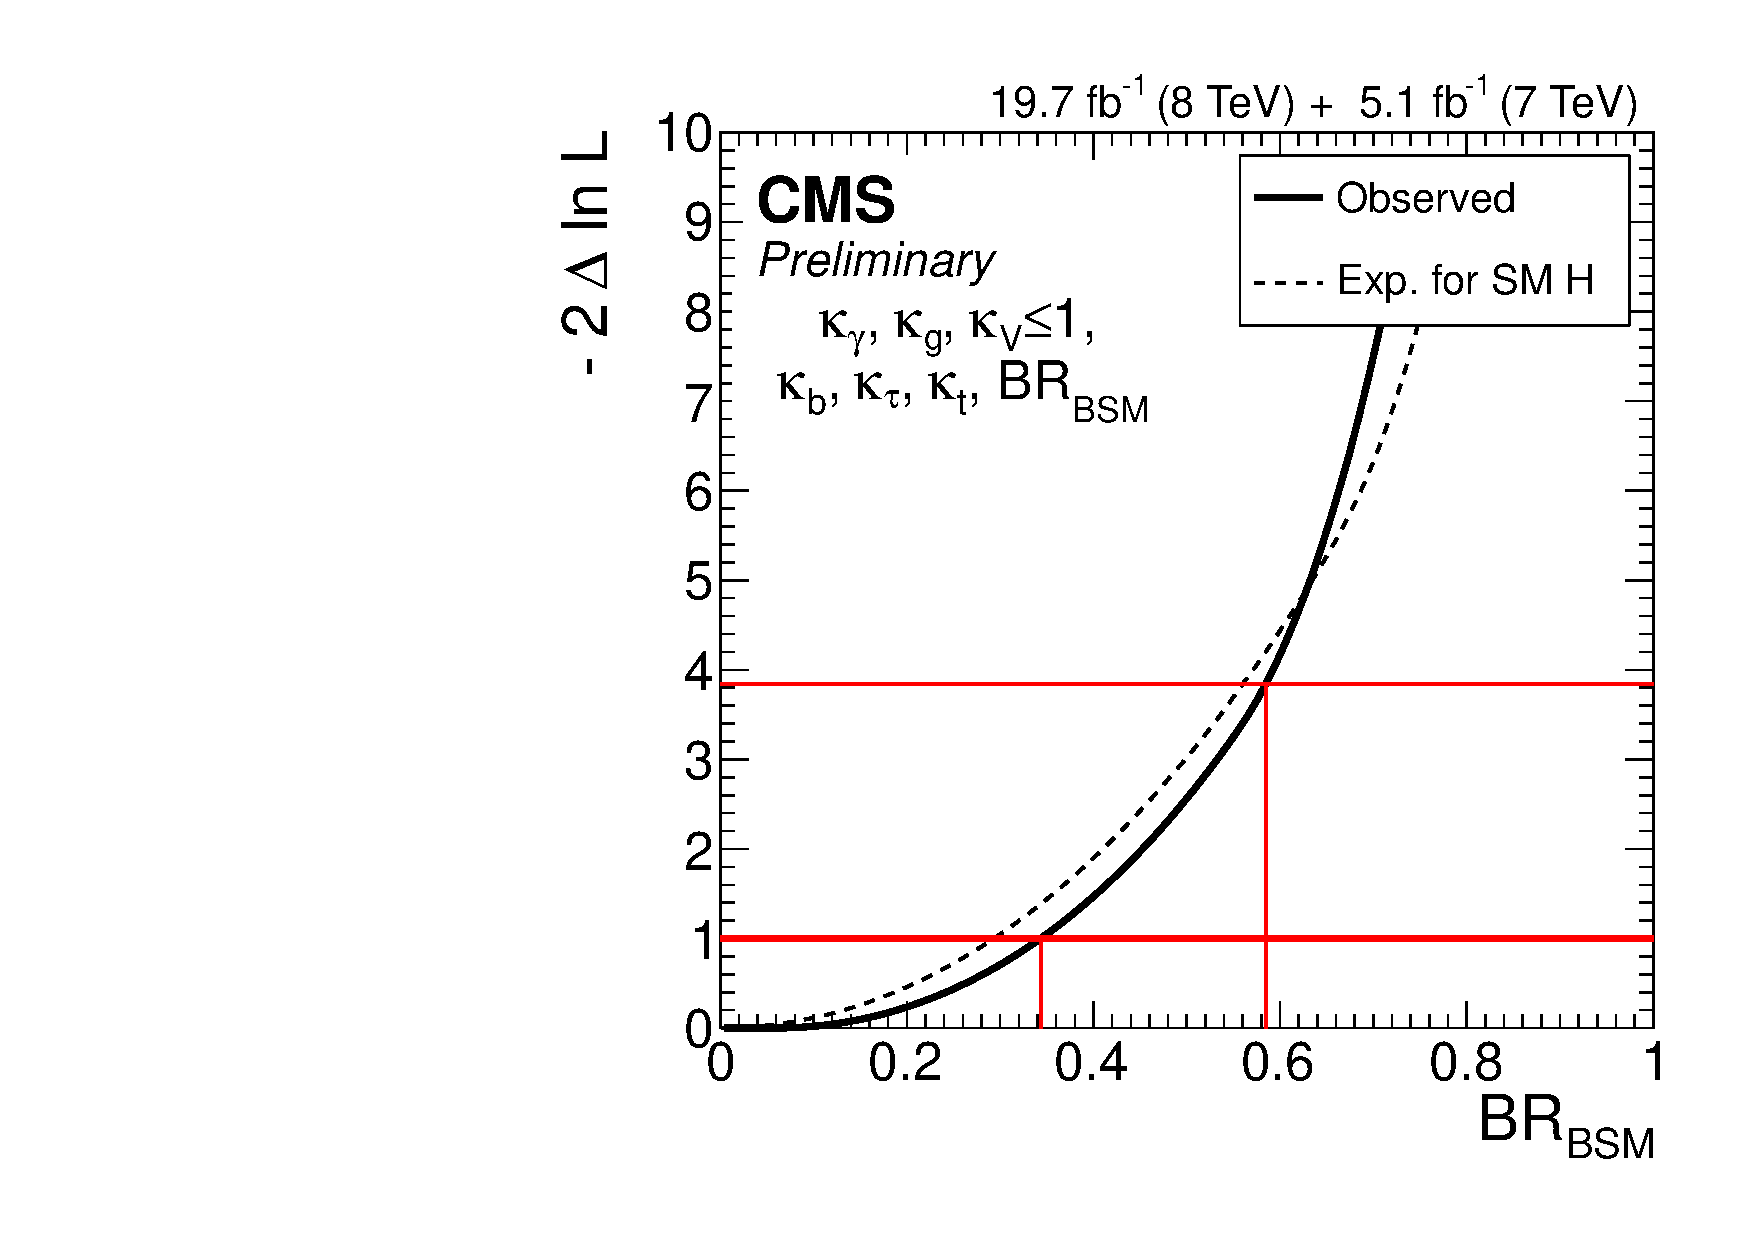
\includegraphics[height=.5\textheight]{TalkPics/panicpics/indirectbrbsm.pdf}
      \column{.05\textwidth}
      \begin{turn}{-90}\scriptsize CMS-PAS-HIG-14-009\end{turn}
        

    \end{columns}
    \vspace{-.5cm}
    \begin{columns}
      \column{.5\textwidth}
      \vspace{-.3cm}
      \begin{block}{\scriptsize Direct searches}
        \scriptsize
        \begin{itemize}
        \item Direct searches must be performed in channels where the Higgs recoils against a visible system
        \item We look in the VBF (left) and ZH (right) channels
        \item[-] For ZH we study the case where the Z decays to two leptons Z($\ell\ell$)H or two b quarks Z(bb)H
        \end{itemize}
      \end{block}
      \column{.01\textwidth}
      \column{.49\textwidth}
      %vbf                                                                                                                                                     
      \begin{fmfgraph*}(60,60)
        \fmfleft{i1,i2}
        \fmfright{o1,o2,o3}
        \fmf{fermion}{i1,v1,o1}
        \fmf{fermion}{i2,v2,o3}
        \fmf{photon,label=$W,,Z$,l.side=left}{v1,v4}
        \fmf{photon}{v4,v3}
        \fmf{photon,label=$W,,Z$,l.side=right}{v2,v5}
        \fmf{photon}{v5,v3}
        \fmf{dashes}{v3,v6}
        \fmf{dashes}{v6,o2}
        \fmflabel{$q$}{i1}
        \fmflabel{$q$}{i2}
        \fmflabel{$q$}{o1}
        \fmflabel{$q$}{o3}
        \fmflabel{$H$}{o2}
      \end{fmfgraph*}
      \hspace{.4cm}
      %zh
      \begin{fmfgraph*}(60,60)
        \fmfleft{i1,i2}
        \fmfright{o1,o2}
        \fmf{fermion}{i1,v1}
        \fmf{fermion}{v1,i2}
        \fmf{photon,label=$W,,Z$}{v1,v2}
        \fmf{photon}{v2,o1}
        \fmf{dashes}{v2,o2}
        \fmflabel{$q$}{i1}
        \fmflabel{$\bar{q}$}{i2}
        \fmflabel{$W,Z$}{o1}
        \fmflabel{$H$}{o2}
      \end{fmfgraph*}
    \end{columns}
  \end{frame}

  \begin{frame}
    \frametitle{VBF outline}
    \vspace{.5cm}
    \begin{columns}
      \column{.56\textwidth}
      \vspace{-.7cm}
      \begin{block}{\scriptsize Signal Topology and Selection}
        \scriptsize
        \begin{itemize}
        \item Two jets with large rapidity separation and missing transverse momentum (MET)
          \ssmall
        \item[-] 2 jets, $p_{T}>50 GeV$, $\eta_{j1}\cdot\eta_{j2}<0$, $\Delta\eta_{jj}>4.2$
        \item[-] $M_{jj}>1100 GeV$, $\Delta\phi_{jj}<1.0$
        \item[-] $MET>130 GeV$
        \end{itemize}
      \end{block}
      \vspace{-.2cm}
      \begin{block}{\scriptsize Backgrounds and Rejection Cuts}
        \scriptsize
        \begin{itemize}
        \item $W\rightarrow \ell\nu$+jets:
          \ssmall
        \item[-]Veto any events with leptons with $p_{T}>10$ GeV
          \scriptsize
        \item $Z\rightarrow\nu\nu$+jets: Irreducible
        \item QCD multijet events:
          \ssmall
        \item[-]Veto events with jets with $p_{T}>30$ GeV between the two selected jets (CJV)
          \scriptsize
        \item Minor backgrounds from: $t\bar{t}$, single top, diboson and $Z\rightarrow \ell\ell$+jets
        \end{itemize}
      \end{block}
      \column{.44\textwidth}
      \centering
      \begin{fmfgraph*}(60,50)
        \fmfleft{i1,i2}
        \fmfright{o1,o2,o3}
        \fmf{fermion}{i1,v1,o1}
        \fmf{fermion}{i2,v2,o3}
        \fmf{photon,label=$W,,Z$,l.side=left}{v1,v4}
        \fmf{photon}{v4,v3}
        \fmf{photon,label=$W,,Z$,l.side=right}{v2,v5}
        \fmf{photon}{v5,v3}
        \fmf{dashes}{v3,v6}
        \fmf{dashes}{v6,o2}
        \fmflabel{$q$}{i1}
        \fmflabel{$q$}{i2}
        \fmflabel{$q$}{o1}
        \fmflabel{$q$}{o3}
        \fmflabel{$H$}{o2}
      \end{fmfgraph*}
      \vspace{.5cm}
      \begin{columns}
        \column{.9\textwidth}
        \hfill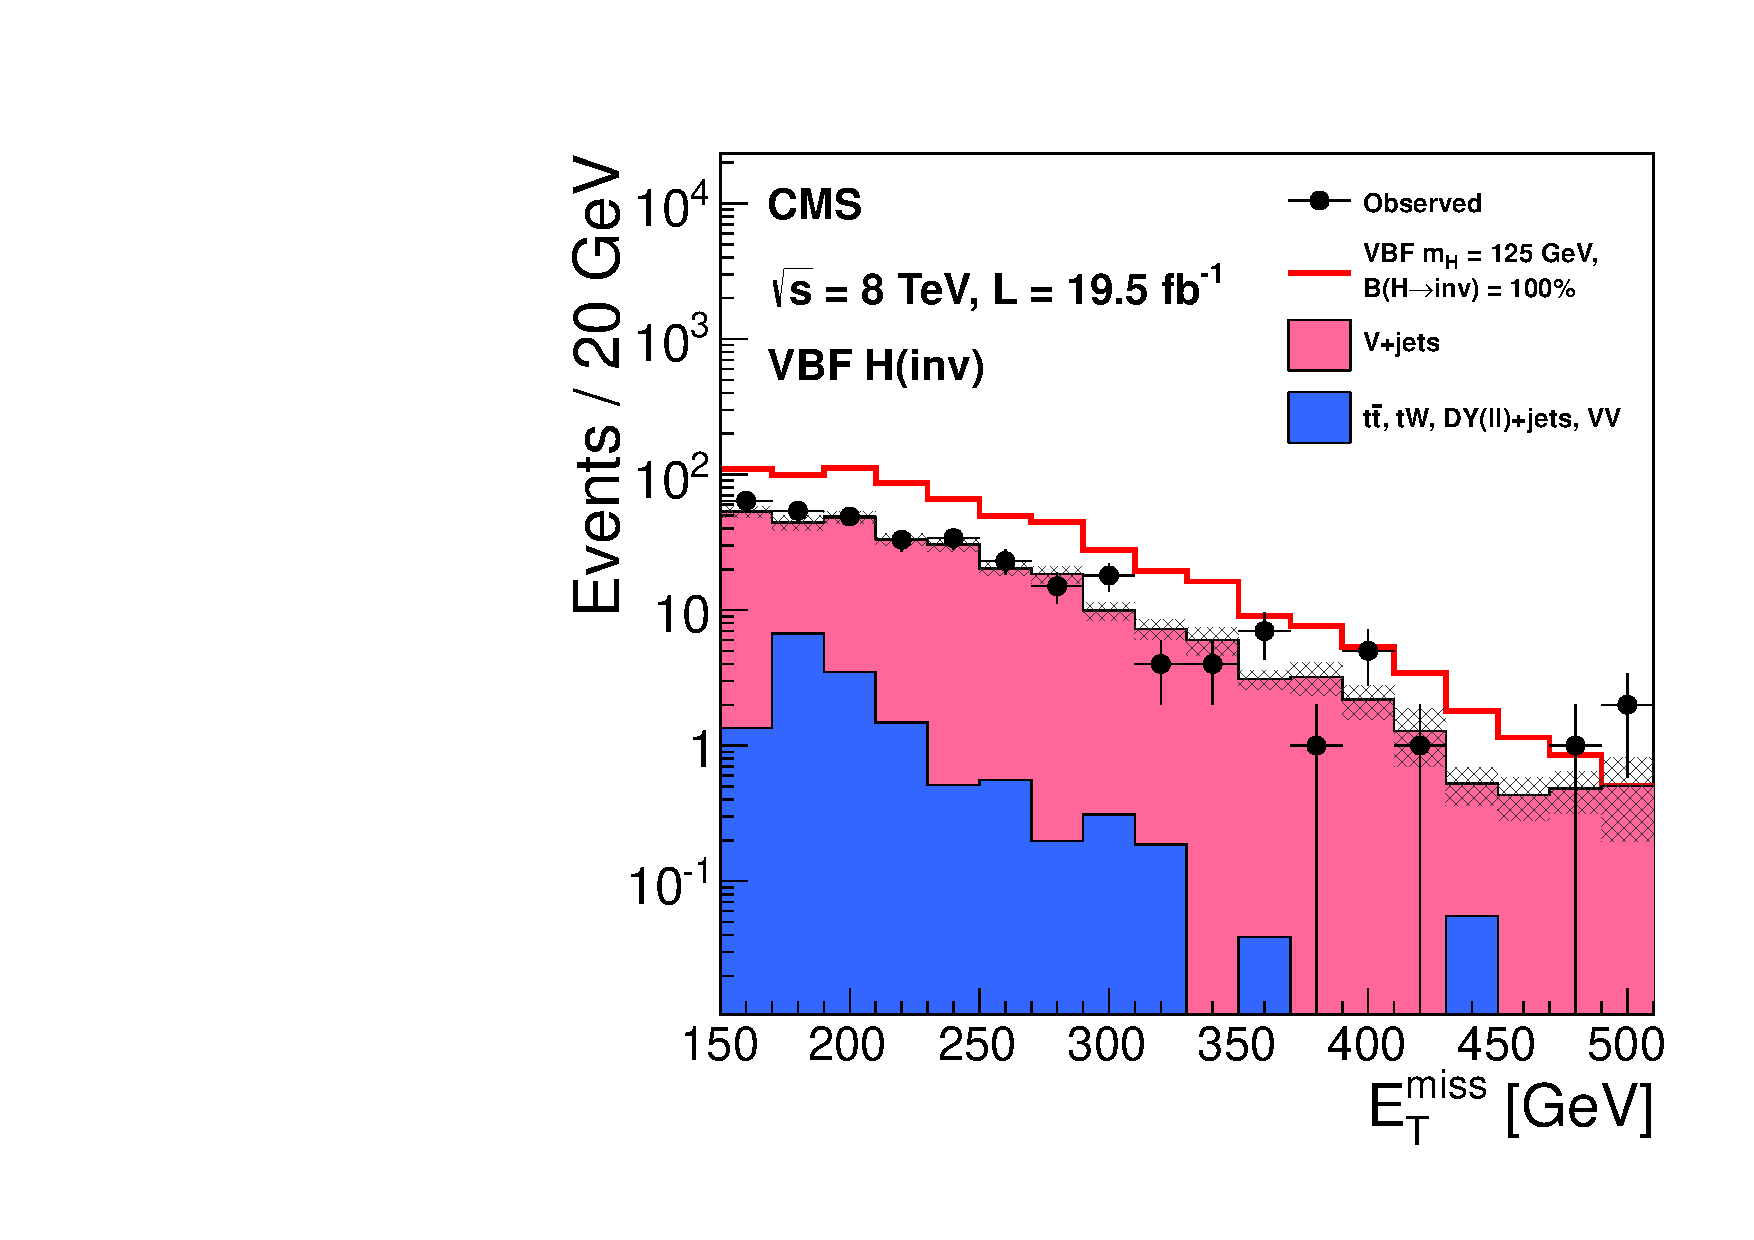
\includegraphics[clip=true,trim=0 0 0 50,height=.55\textheight]{TalkPics/panicpics/vbfmet.pdf}
        \column{.1\textwidth}
        \begin{turn}{-90}\scriptsize arXiv:1404.1344 \end{turn}
      \end{columns}
    \end{columns}
  \end{frame}
  \begin{frame}
    \frametitle{VBF background estimation}
    \begin{columns}
      \column{.6\textwidth}
      \begin{block}{\footnotesize Z+jets - Estimate using $Z\rightarrow\mu\mu$+jets events}
          \scriptsize
        \begin{itemize}
        \item[-] Sig. sel.+two muons 60$<$$m_{\mu\mu}$$<$120 GeV
        \item Control$\rightarrow$signal extrapolation factor from MC
        \item $N_{Z\rightarrow\mu\mu}=99\pm 29(stat.)\pm 25 (syst.)$
        \end{itemize}
      \end{block}
      \begin{block}{\footnotesize W+jets - Estimate using $W\rightarrow\ell\nu$+jets events}
          \scriptsize
          \begin{itemize}
        \item[-] Sig. sel. + require one e/$\mu$/$\tau$
        \item Control$\rightarrow$signal extrapolation factor from MC
        \item $N_{W\rightarrow e\nu}=63\pm 9(stat.)\pm 18 (syst.)$
        \item $N_{W\rightarrow \mu\nu}=67\pm 5(stat.)\pm 16 (syst.)$
        \item $N_{W\rightarrow \tau\nu}=53\pm 18(stat.)\pm 18 (syst.)$
        \end{itemize}
      \end{block}
      \begin{block}{\footnotesize QCD - Use ``ABCD method'' in MET and CJV}
        \scriptsize
        \begin{itemize}
        \item $N_{QCD}=30.9\pm 1.6 (stat.) \pm 23.0 (syst.)$
        \end{itemize}
      \end{block}
      \column{.43\textwidth}
      \begin{columns}
        \vspace{-.3cm}
        \column{.95\textwidth}
        \hfill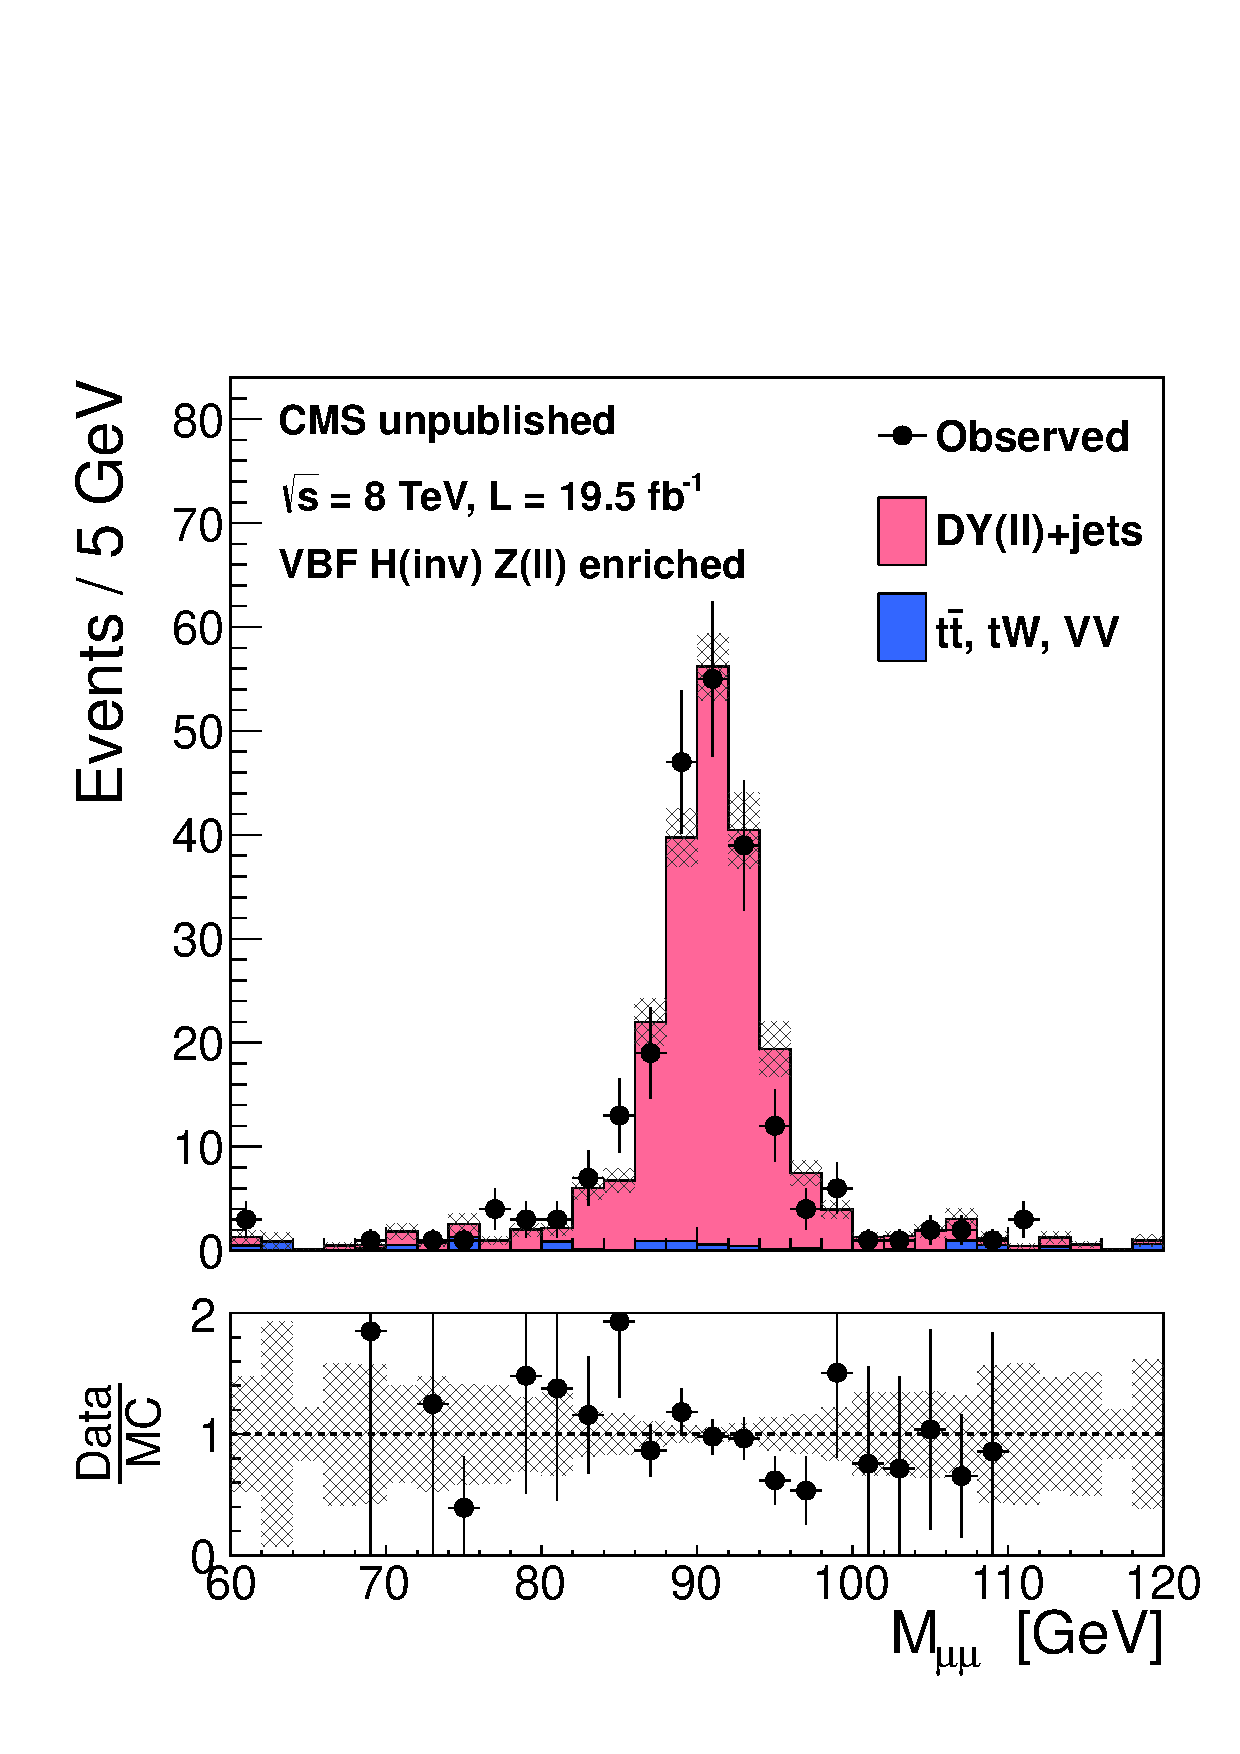
\includegraphics[clip=true,trim=0 0 0 30,height=.65\textheight]{TalkPics/panicpics/vbfzreg.pdf}
        \column{.05\textwidth}
        \hspace{-.7cm}
        \begin{turn}{-90}\scriptsize CMS-TWIKI-HIG-13-030 \end{turn}
      \end{columns}
      \footnotesize
      \centering
      \begin{tabular}{c|c|c|c}
        \multicolumn{1}{c}{CJV} & \multicolumn{1}{c}{} & \multicolumn{1}{c}{} & \multicolumn{1}{c}{} \\
        \cline{2-3}
        pass & \cellcolor{red!50} B &\cellcolor{green!50} A & \\
        \cline{2-3}
        fail & \cellcolor{red!50} D &\cellcolor{red!50} C & \\
        \cline{2-3}
        \multicolumn{1}{c}{}& \multicolumn{1}{c}{$<$130} & \multicolumn{1}{c}{$>$130} & MET
      \end{tabular}
      
    \end{columns}
    
  \end{frame}
  \begin{frame}
    \frametitle{VBF results}
          \scriptsize
          \centering
          \begin{tabular}{lc}
            \hline
            Total background & $332\pm 35 (stat.) \pm 45 (syst.)$ \\ 
            \hline
            VBF H(inv.) assuming B(H$\rightarrow$inv)=100\% &  $210 \pm 30(syst.)$ \\ 
            ggF H(inv.) assuming B(H$\rightarrow$inv)=100\%& $14 \pm 11 (syst.)$ \\
            \hline
            Observed data & 390 \\
            \hline
          \end{tabular}
\vspace{-.3cm}
    \begin{columns}
      \column{1.1\textwidth}
          \begin{block}{}
            \scriptsize
            \begin{itemize}
            \item Set limits on $\sigma$x$B(H\rightarrow inv)$
              \vspace{-.1cm}
            \item[-] Perform a single bin counting experiment using $CL_{S}$ method
            \item Assuming SM Higgs production cross-section and acceptance:
              \vspace{-.1cm}
            \item[-]  observed(expected) 95\% C.L. limit on $B(H\rightarrow inv)$ for $m_{H}$=125 GeV is 65(49)\%
            \end{itemize}
          \end{block}
    \end{columns}

    \begin{columns}
      \column{.03\textwidth}
      \column{.55\textwidth}
      \begin{columns}
        \column{.9\textwidth}
      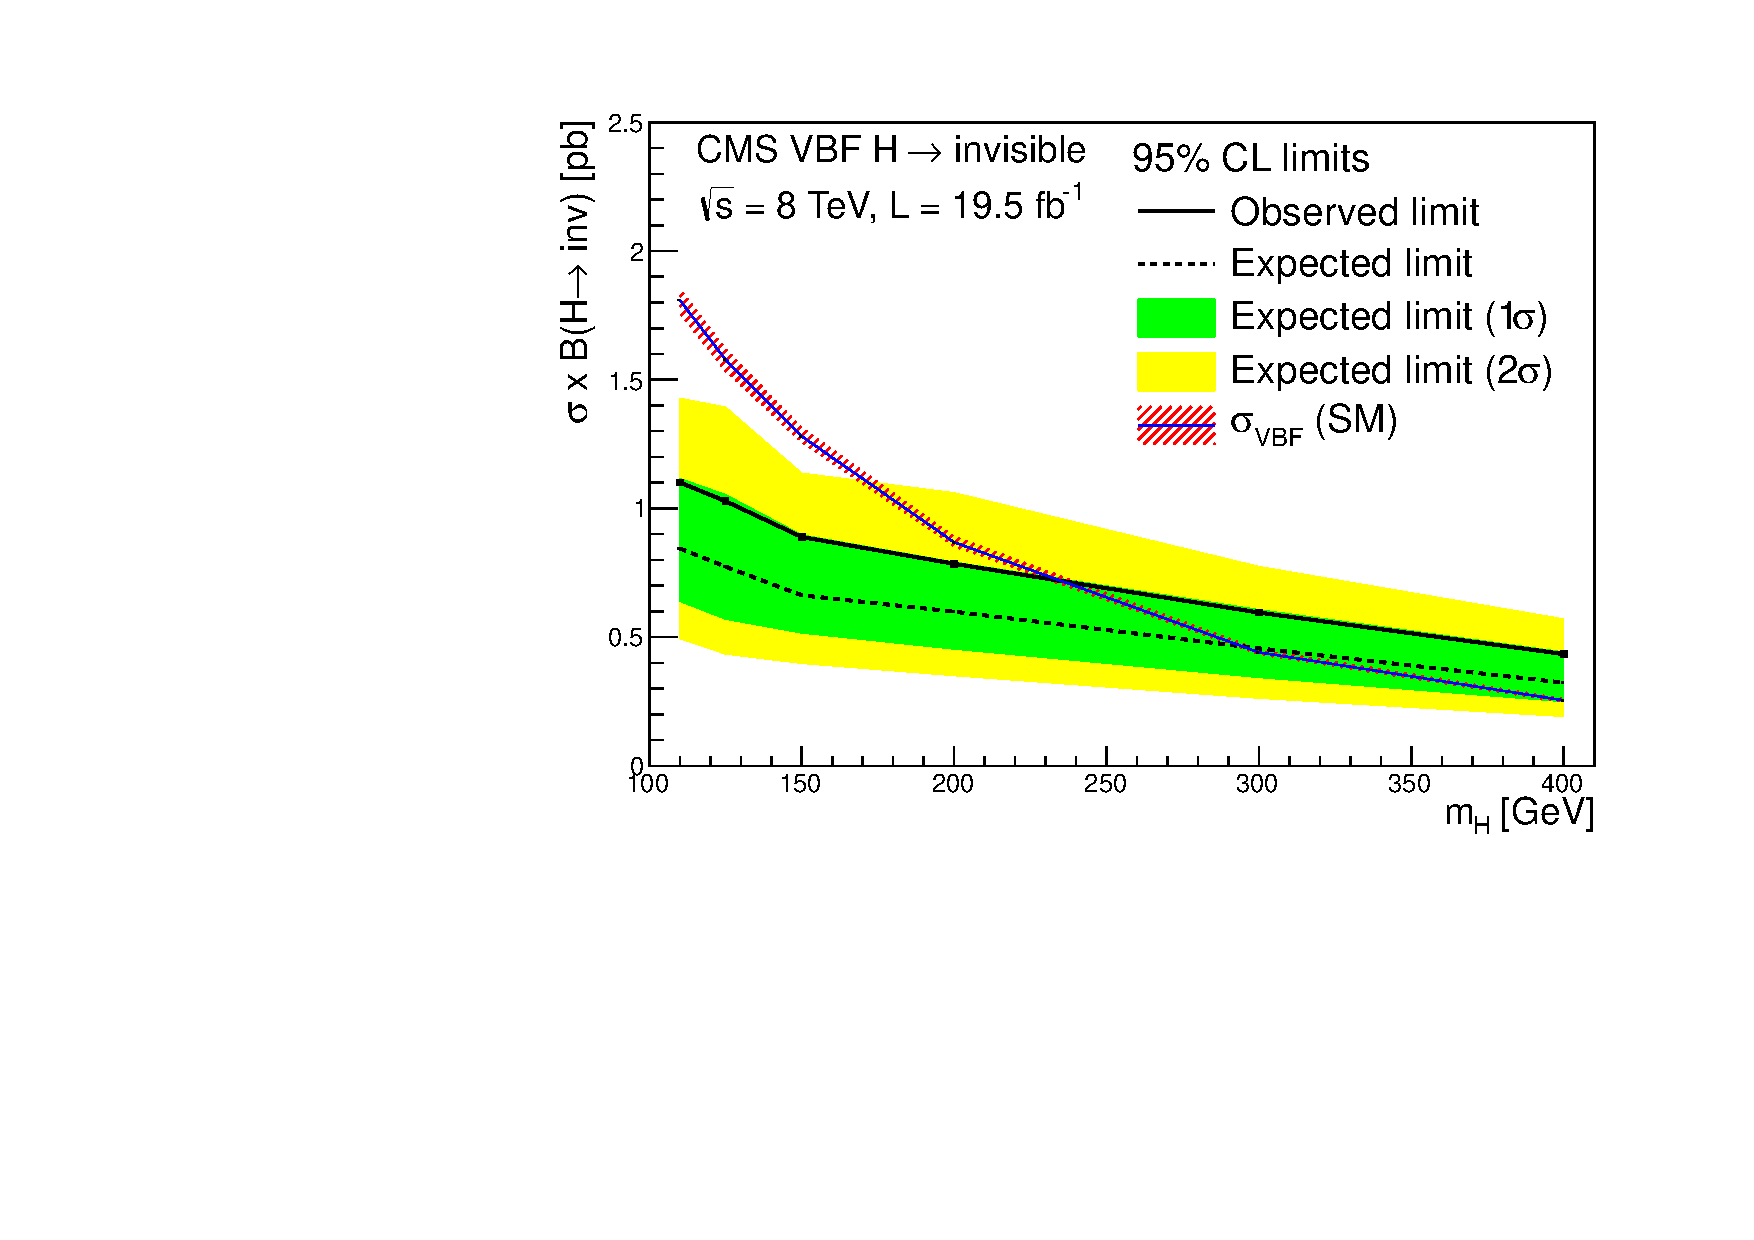
\includegraphics[clip=true,trim=0 0 0 20,width=1.1\textwidth]{TalkPics/panicpics/vbfxslimit.pdf}
      \column{.1\textwidth}
      \hspace{-.5cm}
      \begin{turn}{-90}\scriptsize arXiv:1404.1344 \end{turn}
      \end{columns}
      \column{.55\textwidth}
      \begin{columns}
        \column{.9\textwidth}
      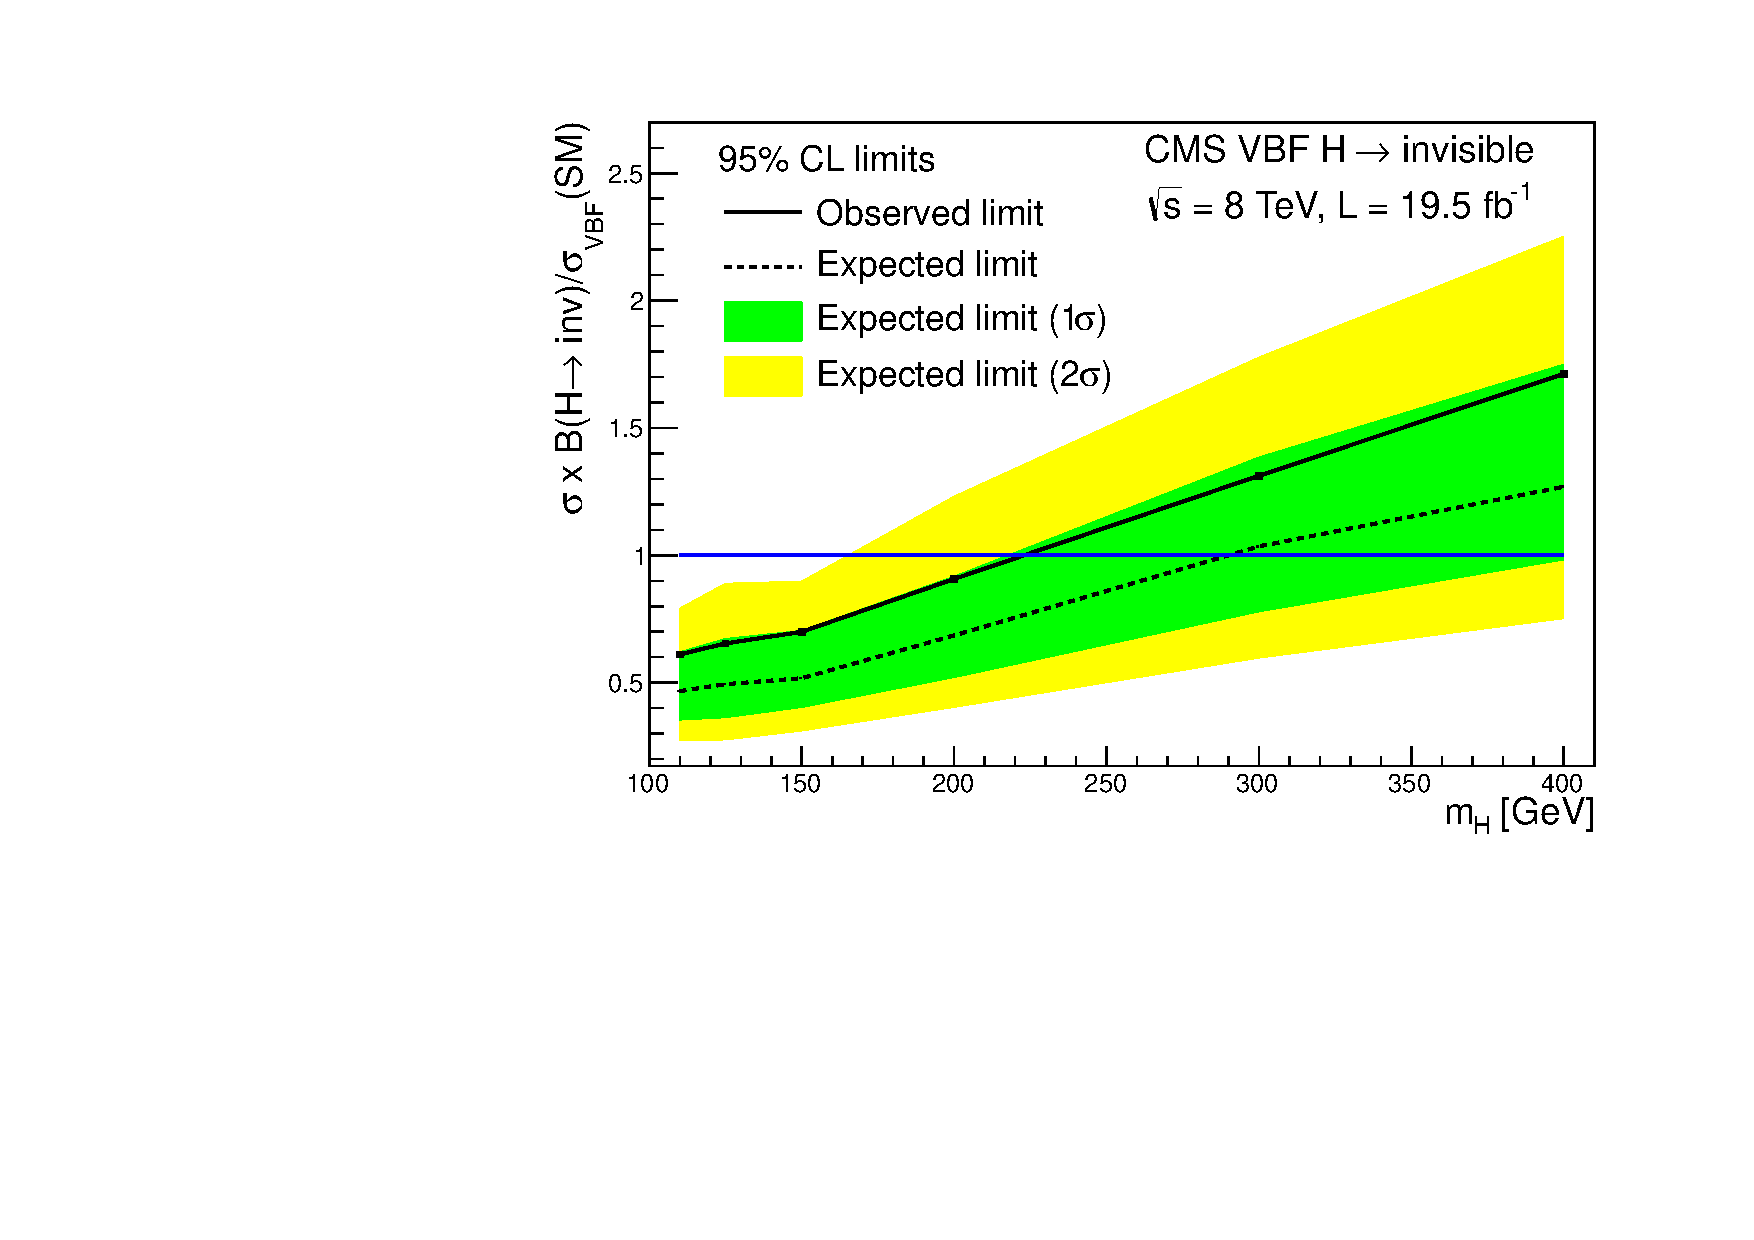
\includegraphics[clip=true,trim=0 0 0 20,width=1.1\textwidth]{TalkPics/panicpics/vbflimit.pdf}
      \column{.1\textwidth}
      \hspace{-.5cm}
      \begin{turn}{-90}\scriptsize arXiv:1404.1344 \end{turn}
      \end{columns}
    \end{columns}
  \end{frame}

  \begin{frame}
    \frametitle{Z($\ell\ell$)H outline}
    \begin{columns}
      \column{.56\textwidth}
      \vspace{-.5cm}
      \begin{block}{\scriptsize Signal Topology and Selection}
        \scriptsize
        \begin{itemize}
        \item Two same flavour opposite sign electrons or muons
          \ssmall
        \item[-] $p_{T}>20$ GeV, $|M_{\ell\ell}-m_{Z}|<15$ GeV
          \scriptsize
        \item Large MET
          \ssmall
        \item[-] $MET>120$ GeV
        \end{itemize}
      \end{block}
      \begin{block}{\scriptsize Backgrounds and Rejection Cuts}
        \scriptsize
        \begin{itemize}
        \item ZZ($\ell\ell\nu\nu$)+jets, WW($\ell\nu\ell\nu$)+jets
        \item WZ($\ell\nu\ell\ell$)+jets
          \ssmall
        \item[-] Veto events with $>$3 leptons, $p_{T}$$>$10 GeV
          \scriptsize
        \item Z($\ell\ell$)+jets
          \ssmall
        \item[-] MET cut, MET-$\ell\ell$ balance requirement
          \scriptsize
        \item $t\bar{t}$, single top, W($\ell\nu$), QCD
          \ssmall
        \item[-] $\leq$1 jet, $p_{T}$$>$30 GeV
        \item[-] no b-tagged jets, $p_{T}>30$ GeV
        \end{itemize}
      \end{block}
      \column{.44\textwidth}
      \centering
      \begin{fmfgraph*}(75,40)
        \fmfleft{i1,i2}
        \fmfright{o1,o2,o3}
        \fmf{fermion}{i1,v1,i2}
        \fmf{photon,label=$Z$}{v1,v2}
        \fmf{photon}{v2,v4}
        \fmf{photon,label=$Z$,l.side=right}{v4,v3}
        \fmf{fermion}{o1,v3,o2}
        \fmf{photon}{v5,v3}
        \fmf{dashes,label=$H$,l.side=left}{v2,o3}
        \fmflabel{$\ell^{+}$}{o1}
        \fmflabel{$\ell^{-}$}{o2}
        \fmflabel{$q$}{i1}
        \fmflabel{$\bar{q}$}{i2}
      \end{fmfgraph*}
      \vspace{.4cm}
      \begin{columns}
        \column{.05\textwidth}
        \column{.9\textwidth}
        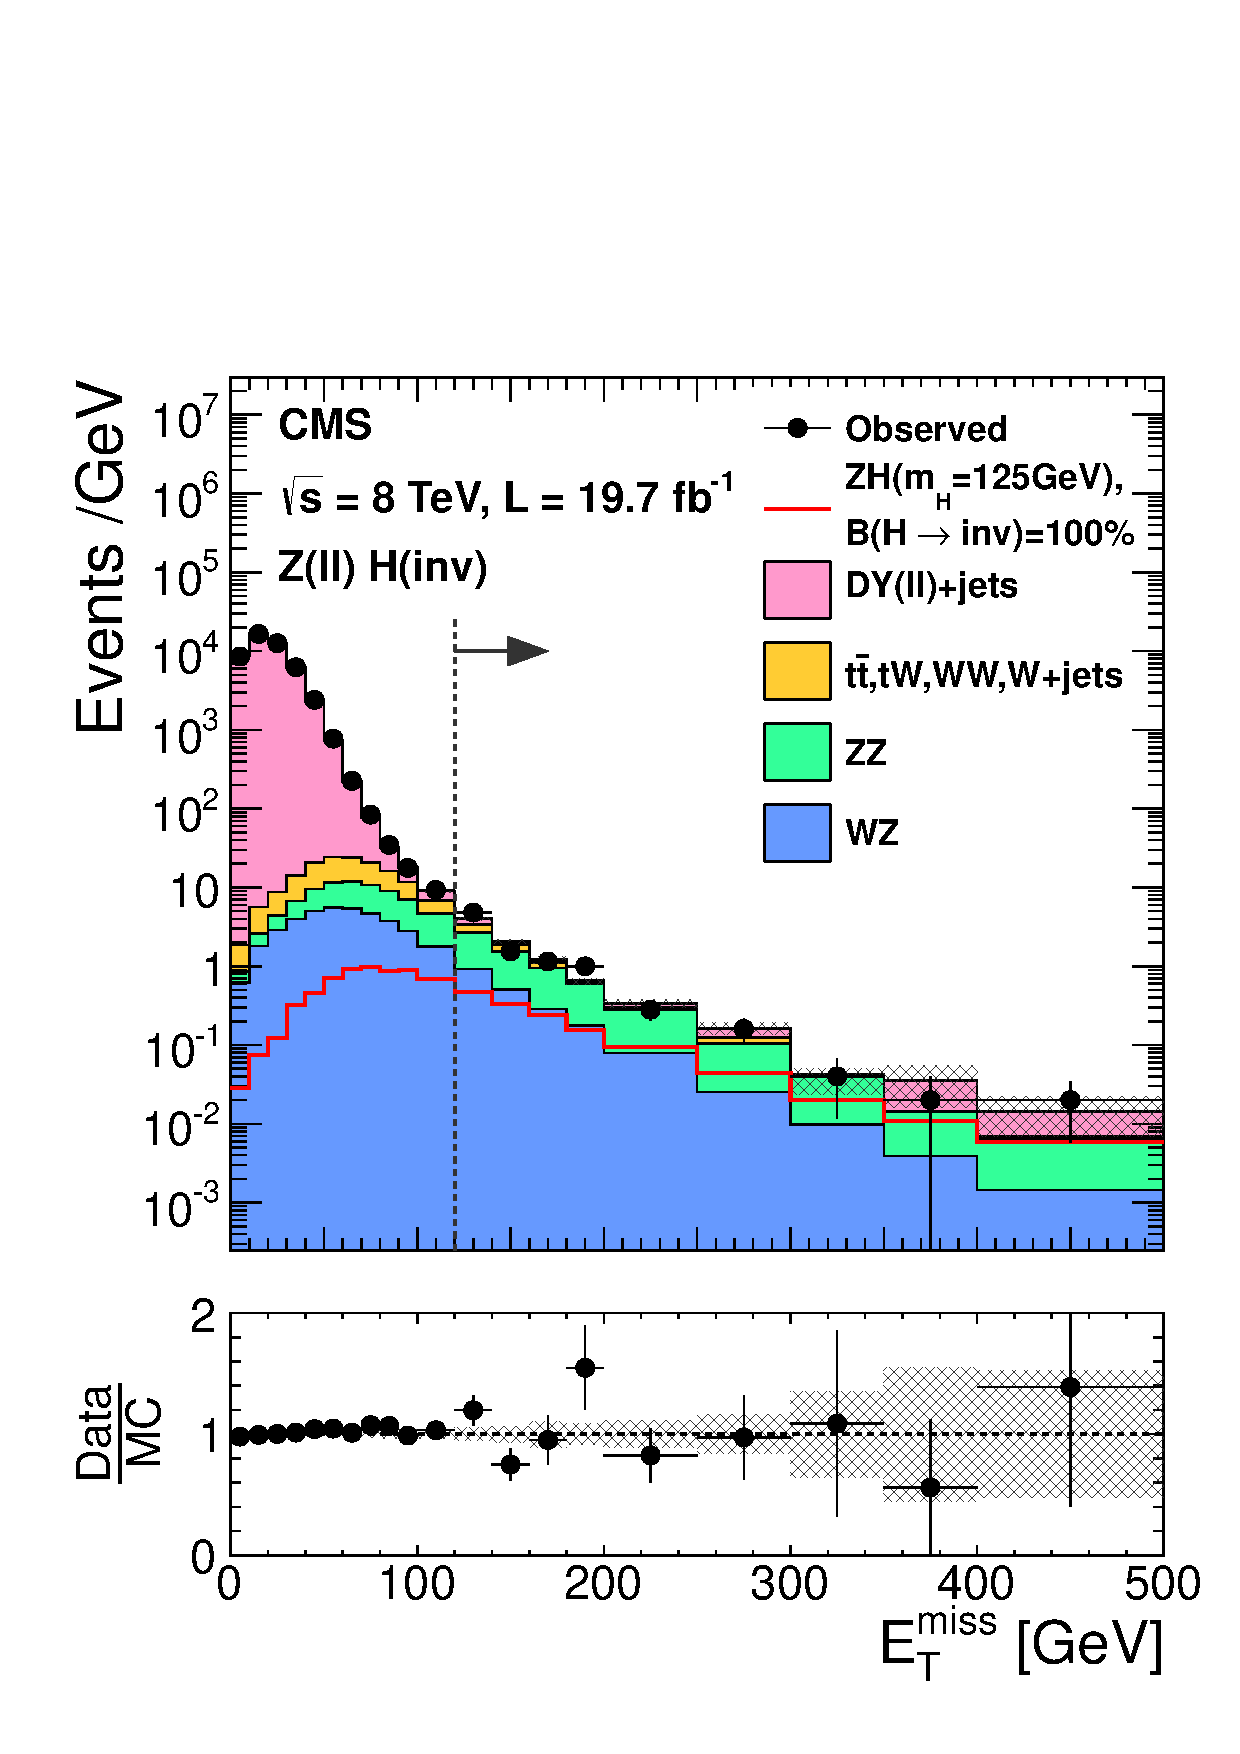
\includegraphics[clip=true,trim=0 0 0 20, width=\textwidth]{TalkPics/panicpics/zllmet.pdf}
        \column{.1\textwidth}
        \hspace{-.4cm}\begin{turn}{-90}\scriptsize arXiv:1404.1344 \end{turn}
      \end{columns}
    \end{columns}

  \end{frame}
  \begin{frame}
    \frametitle{ Z($\ell\ell$)H background estimation}
    \vspace{-.25cm}
    \begin{columns}
      \column{1.06\textwidth}
    \begin{block}{\scriptsize ZZ($\ell\ell\nu\nu$)+jets and WZ($\ell\nu\ell\ell$+jets)}
      \scriptsize
      \begin{itemize}
      \item Estimated from MC prediction
      \end{itemize}
    \end{block}
    \end{columns}
    \vspace{.2cm}
    \begin{columns}
      \column{.5\textwidth}
    \begin{block}{\scriptsize Z($\ell\ell$)+jets}
      \scriptsize
      \begin{itemize}
      \item Estimated from photon + jets events
      \item[-] Photon $p_{T}$ spectrum reweighted to match Z spectrum
      \end{itemize}
    \end{block}
      \column{.5\textwidth}
      \begin{columns}
        \column{.5\textwidth}
        \centering
      \begin{fmfgraph*}(50,40)
        \fmfleft{i1,i2}
        \fmfright{o1,o2,o3}
        \fmf{gluon}{i2,v1}
        \fmf{fermion}{i1,v1,v2,o3}
        \fmf{photon}{v2,v4}
        \fmf{photon,label=$Z$,l.side=right}{v4,v5}
        \fmf{fermion}{o1,v5,o2}
        \fmflabel{$q$}{i1}
        \fmflabel{$q$}{o3}
        \fmflabel{$g$}{i2}
        \fmflabel{$\ell^{-}$}{o2}
        \fmflabel{$\ell^{+}$}{o1}
      \end{fmfgraph*}
      \column{.5\textwidth}
      \centering
      \begin{fmfgraph*}(50,40)
        \fmfleft{i1,i2}
        \fmfright{o1,o2}
        \fmf{gluon}{i2,v1}
        \fmf{fermion}{i1,v1,v2,o2}
        \fmf{photon}{v2,v4}
        \fmf{photon}{v4,o1}
        \fmflabel{$q$}{i1}
        \fmflabel{$q$}{o2}
        \fmflabel{$g$}{i2}
        \fmflabel{$\gamma$}{o1}
      \end{fmfgraph*}
      \end{columns}
    \end{columns}
    \begin{columns}
      \column{1.06\textwidth}
    \begin{block}{\scriptsize WW($\ell\nu\ell\nu$)+jets, single top, $t\bar{t}$, $Z(\tau\tau$)}
      \scriptsize
      \begin{itemize}
      \item Estimated from $e\mu$ events and Z peak sidebands:
        \ssmall
        \vspace{-.1cm}
      \item[-] $m_{\ell\ell}$ 40-70 and 110-200 GeV
        \scriptsize
      \item[-] $N_{\ell\ell}^{sig}=N^{sig}_{e\mu}\cdot N_{\ell\ell}^{SB}/N_{e\mu}^{SB}$

      \end{itemize}
    \end{block}
    \end{columns}
  \end{frame}

  \begin{frame}
    \frametitle{Z($\ell\ell$)H results}
    \vspace{-.2cm}
      \vspace{-.2cm}
    \begin{block}{}
      \tiny
      \centering
      \begin{tabular}{cccccc}
        \hline
        \vspace{-.05cm}
        & Process & \multicolumn{2}{c}{$\sqrt{s}=7$TeV} & \multicolumn{2}{c}{$\sqrt{s}=8$TeV} \\
        \vspace{-.05cm}
        & & ee & $\mu\mu$ & ee & $\mu\mu$ \\
        \hline
        \vspace{-.05cm}
        0 jets & Total backgrounds & $8.7\pm 6.5$ & $11.0\pm 3.3$ & $37.4\pm 3.7$ & $51.6\pm 4.8$ \\
        & ZH(125) & $2.3\pm 0.2$ & $3.1\pm 0.3$ & $10.3\pm 1.2$ & $14.7\pm 1.5$ \\
        & Observed data & 9 & 10 & 36 & 46 \\
        \hline
        & S/B for B(H$\rightarrow$inv) 100\% & 0.26 & 0.28 & 0.28 & 0.24 \\ 
        \hline
        1 jet & Total backgrounds & $2.6\pm 0.7$ & $2.8\pm 0.9$ & $10.6\pm 4.2$ & $13.8\pm 5.8$ \\
        & ZH(125) & $0.4\pm 0.1$ & $0.5\pm 0.1$ & $1.6\pm 0.2$ & $2.5\pm 0.3$ \\
        & Observed data & 1 & 4 & 11 & 17  \\
        \hline
        & S/B for B(H$\rightarrow$inv) 100\% & 0.15  & 0.18 & 0.15 & 0.18 \\ 
        \hline
      \end{tabular}
      \end{block}
    \vspace{-.4cm}
    \begin{columns}
      \column{.4\textwidth}
      \column{.3\textwidth}
    \scriptsize arXiv:1404.1344
    \vspace{-.2cm}
      \column{.3\textwidth}
    \scriptsize arXiv:1404.1344
    \vspace{-.2cm}
    \end{columns}
    \begin{columns}
      \column{1.05\textwidth}
    \begin{columns}
     \column{.4\textwidth}
     \hspace{.1cm}
     \begin{block}{}
       \scriptsize
       \begin{itemize}
       \item Limits obtained from a 2D fit to $m_{T}$ and $\Delta\phi (\ell\ell)$
       \item[-] 1D fit to $m_{T}$ for 7 TeV data
       \item Assuming SM Higgs production cross-section and acceptance:
       \item[-]  observed(expected) 95\% C.L. limit on $B(H\rightarrow inv)$ for $m_{H}$=125 GeV is 83(86)\%
       \end{itemize}

    \end{block}
     \column{.29\textwidth}
     \begin{columns}

       \column{.95\textwidth}
       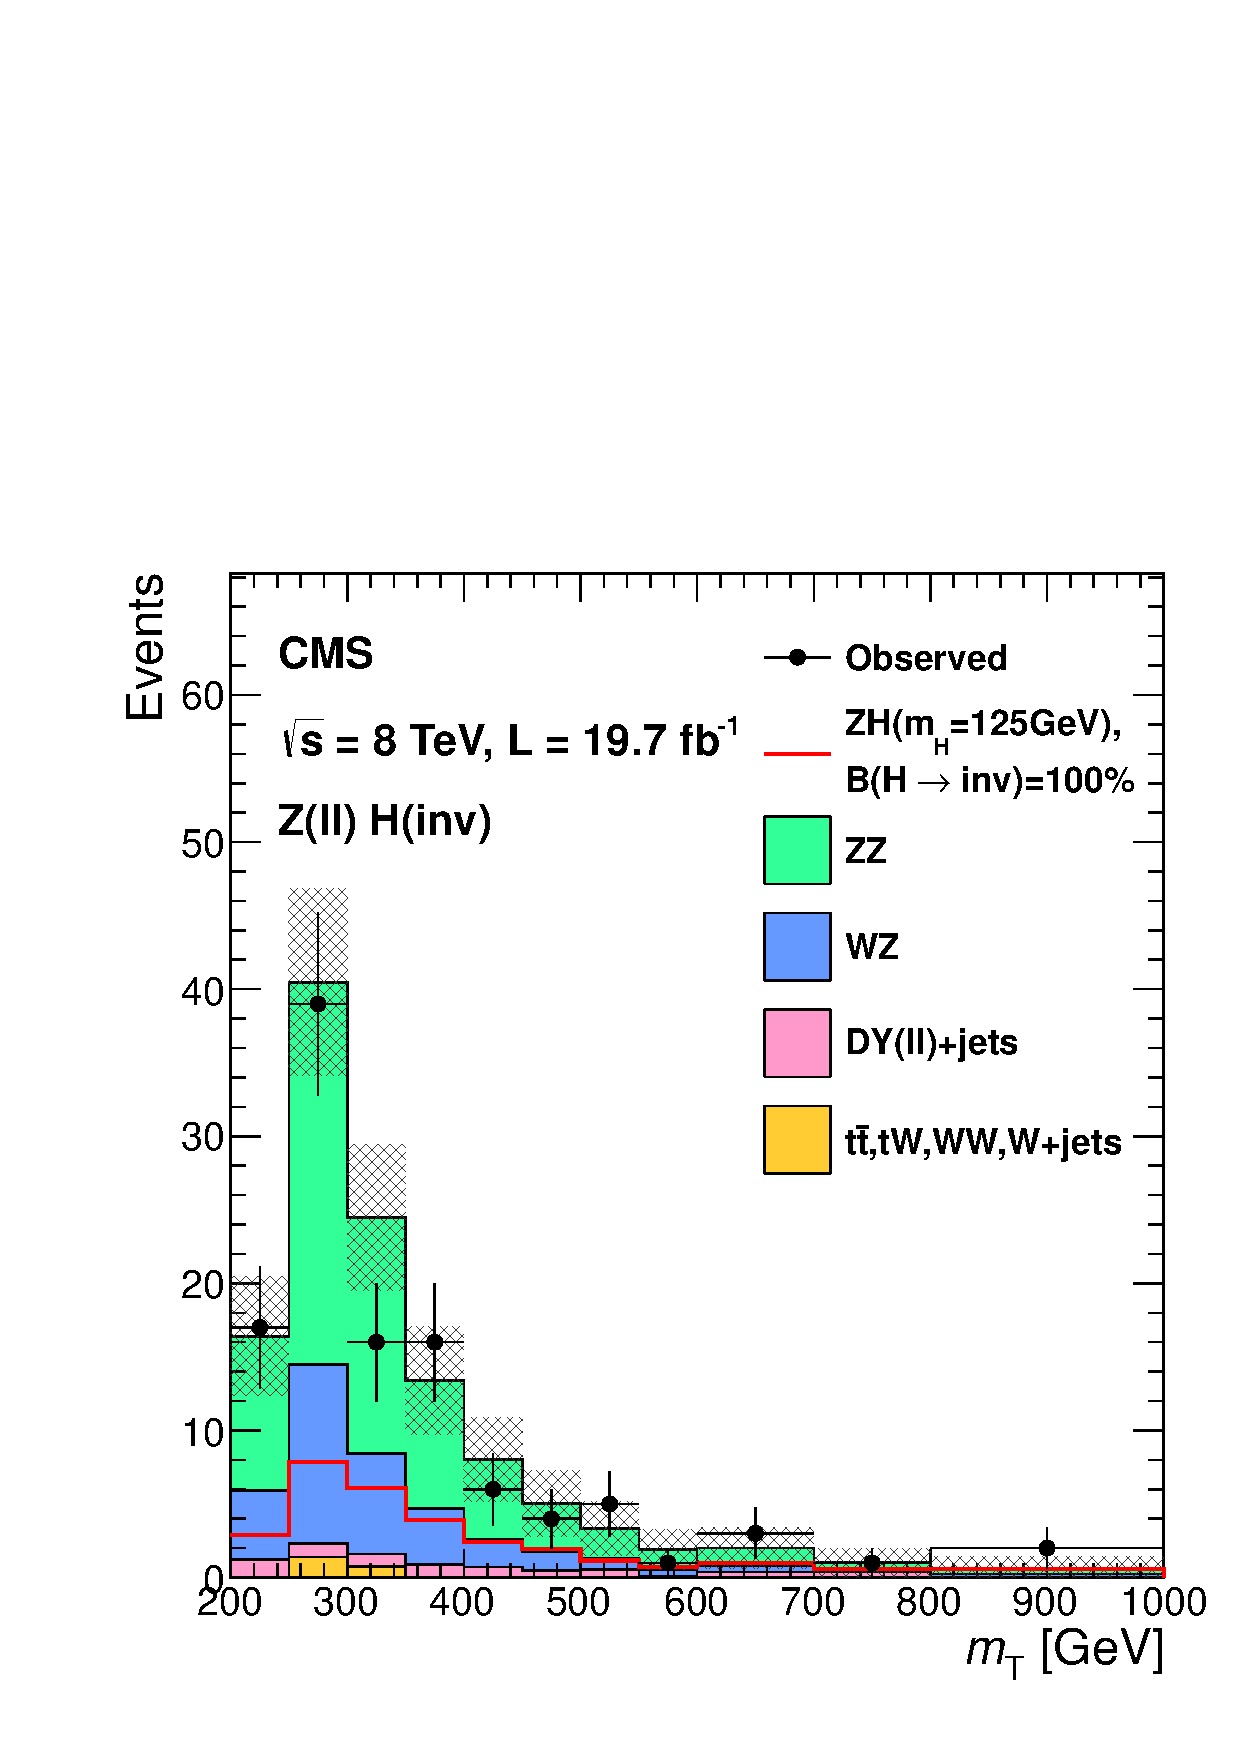
\includegraphics[clip=true,trim=25 0 0 20, height=.53\textheight]{TalkPics/panicpics/zllmt.pdf}
       \column{.06\textwidth}

     \end{columns}
    \column{.29\textwidth}
     \begin{columns}
       \column{.95\textwidth}
       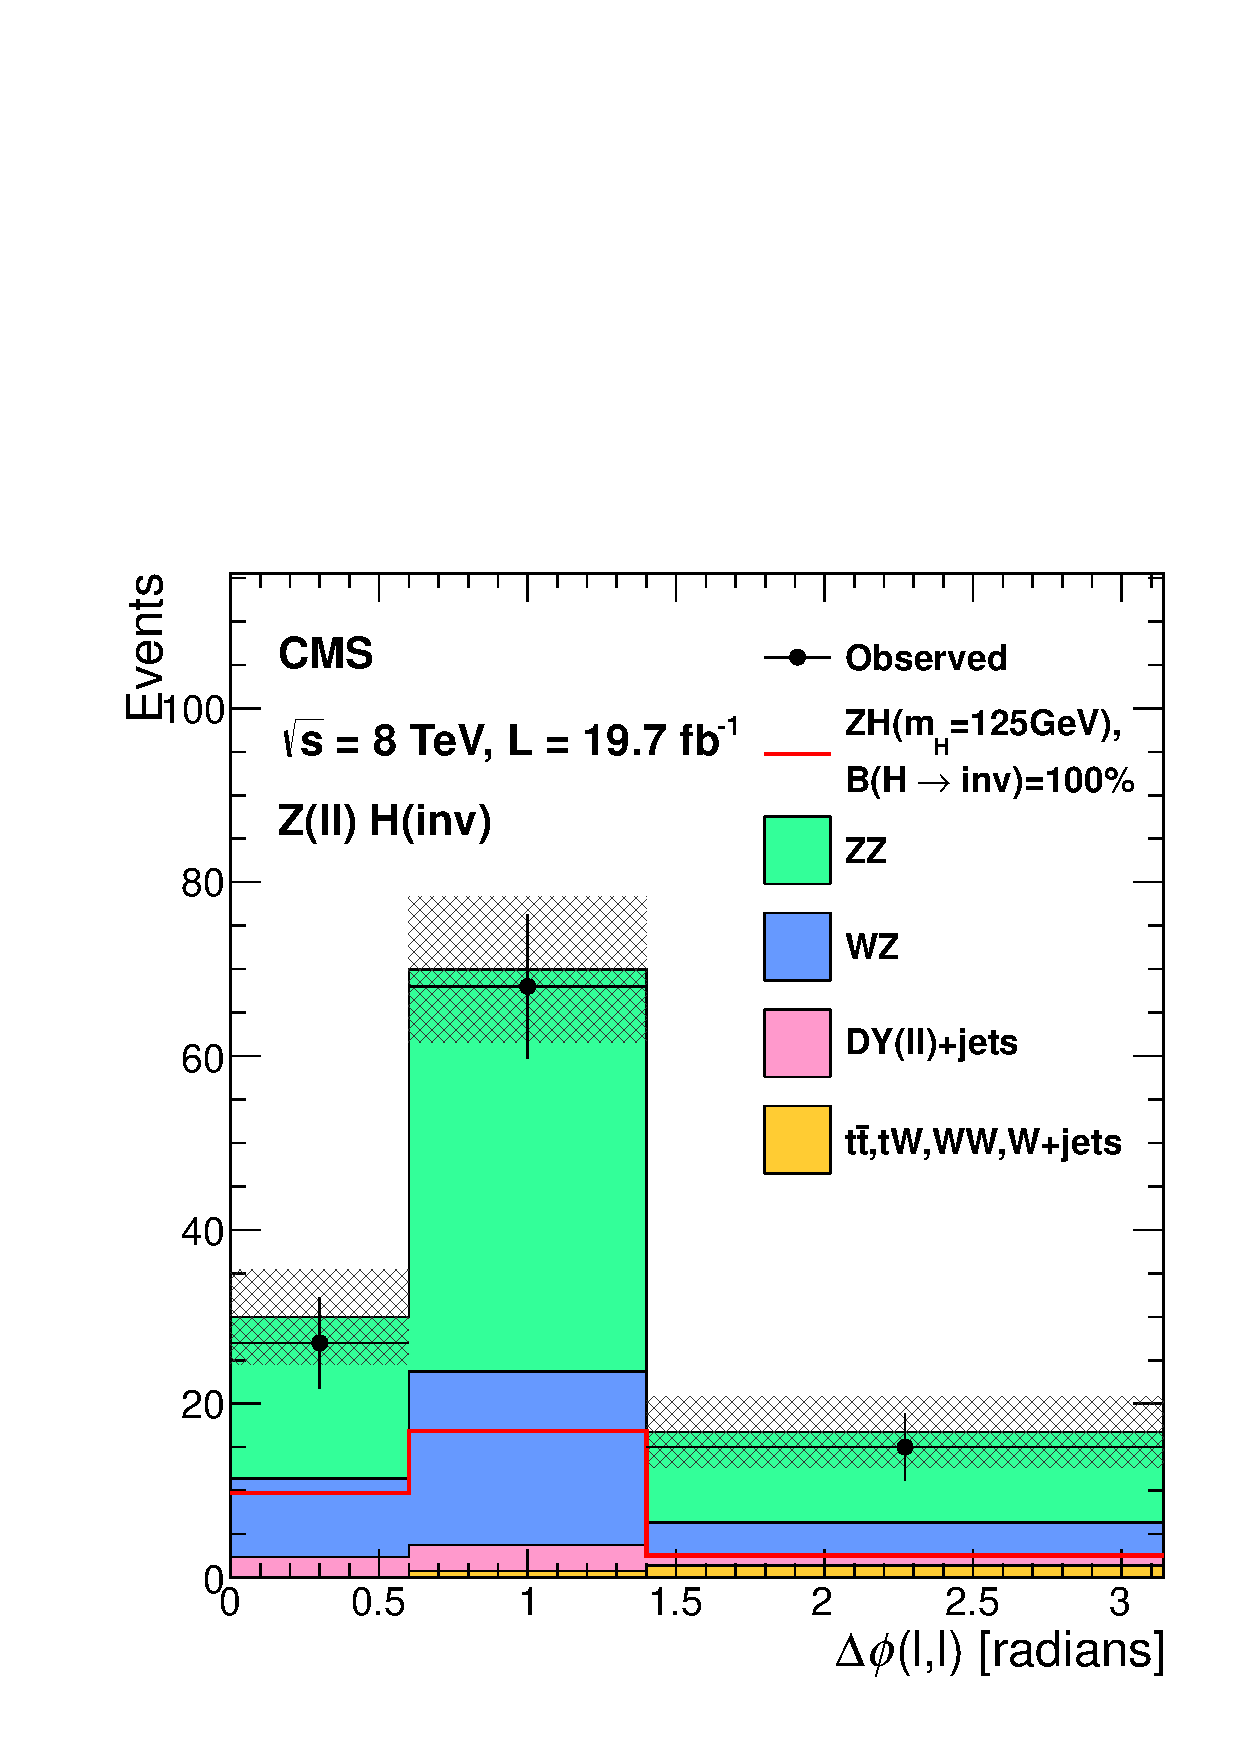
\includegraphics[clip=true,trim=25 0 0 20, height=.53\textheight]{TalkPics/panicpics/zlldphi.pdf}
       \column{.05\textwidth}
     \end{columns}


    \end{columns}
    \end{columns}
  \end{frame}


  \begin{frame}
    \frametitle{Z(bb)H outline and backgrounds}
    \vspace{.4cm}
    \begin{columns}
      \column{.56\textwidth}
      \vspace{-.82cm}
      \begin{block}{\scriptsize Signal Topology and Selection}
        \scriptsize
        \begin{itemize}
          \vspace{-.05cm}
        \item Two b-tagged jets:
          \vspace{-.05cm} 
         \ssmall
        \item[-]$p_{T}>30/60$ GeV, $p_{Tjj}>100-130$ GeV
            \scriptsize
        \item Three bins in MET
          \vspace{-.05cm}
          \ssmall
        \item[-] 100-130, 130-170, $>170$ GeV
                  \end{itemize}
      \end{block}
      \vspace{-.15cm}
      \begin{block}{\scriptsize Backgrounds and Rejection Cuts}
        \scriptsize
        \begin{itemize}
          \vspace{-.05cm}
        \item Z($\nu\nu$)+jets, W($\ell\nu$)+jets
          \vspace{-.05cm}
        \item ZZ($\nu\nu b\bar{b}$)
          \vspace{-.05cm}
        \item WZ($\ell\nu b\bar{b}$), $t\bar{t}$, single top
          \vspace{-.05cm}
          \ssmall
        \item[-] Veto events with leptons, $p_{T}$$>$15 GeV
          \scriptsize
          \vspace{-.05cm}
        \item QCD
          \vspace{-.05cm}
          \ssmall
        \item[-] MET quality requirements
          \vspace{-.05cm}
        \end{itemize}
      \end{block}
      \vspace{-.15cm}
      \begin{block}{\scriptsize Background estimation - data normalised MC}
        \scriptsize
        \begin{itemize}
          \vspace{-.05cm}
        \item Normalisation from a simultaneous fit in seven control regions:
          \vspace{-.05cm}
          \ssmall
        \item[-] Z+jets (0,1,2 b-jets), W+jets (0,1,2 b-jets), $t\bar{t}$
          \vspace{-.05cm}
          
        \end{itemize}
      \end{block}
      \column{.44\textwidth}
      \centering
      \begin{fmfgraph*}(75,40)
        \fmfleft{i1,i2}
        \fmfright{o1,o2,o3}
        \fmf{fermion}{i1,v1,i2}
        \fmf{photon,label=$Z$}{v1,v2}
        \fmf{photon}{v2,v4}
        \fmf{photon,label=$Z$,l.side=right}{v4,v3}
        \fmf{fermion}{o1,v3,o2}
        \fmf{photon}{v5,v3}
        \fmf{dashes,label=$H$,l.side=left}{v2,o3}
        \fmflabel{$\bar{b}$}{o1}
        \fmflabel{$b$}{o2}
        \fmflabel{$q$}{i1}
        \fmflabel{$\bar{q}$}{i2}
      \end{fmfgraph*}
      \vspace{.45cm}
      \begin{columns}
        \column{.05\textwidth}
        \column{.9\textwidth}
        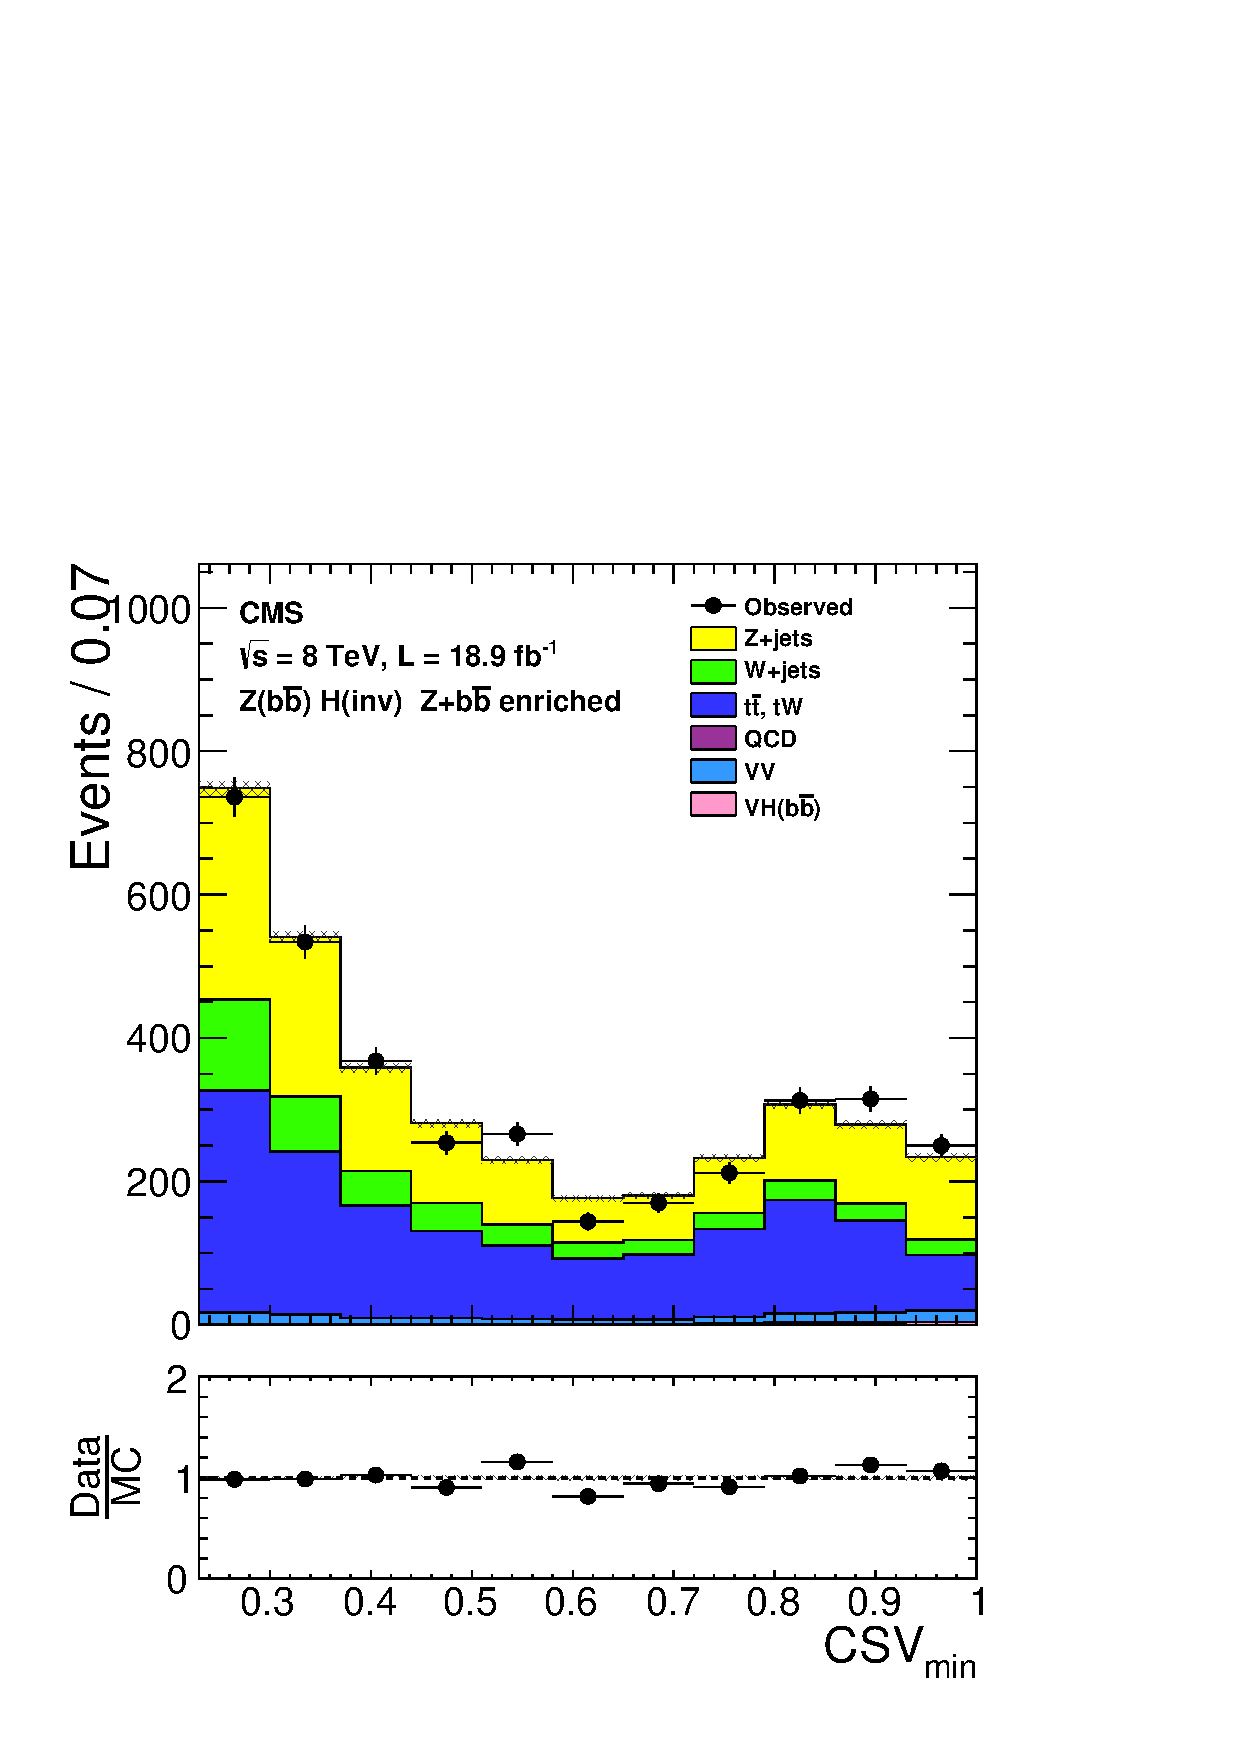
\includegraphics[clip=true,trim=0 0 0 20, width=.95\textwidth]{TalkPics/panicpics/zbbcsv.pdf}
        \column{.1\textwidth}
        \hspace{-.4cm}\begin{turn}{-90}\scriptsize arXiv:1404.1344 \end{turn}
      \end{columns}
    \end{columns}


  \end{frame}

  \begin{frame}
    \frametitle{Z($b\bar{b}$)H results}
    \vspace{-.2cm}
    \begin{columns}
      \column{.7\textwidth}
    \begin{block}{}
      \centering
      \tiny
      \begin{tabular}{lccc}
        \hline
        Process & High $p_{T}(V)$ & Intermediate $p_{T}(V)$ & Low $p_{T}(V)$ \\
        \hline
        Total backgrounds & $181.3\pm 9.8$ & $64.8\pm 4.1$ & $40.5\pm 4.1$ \\
        Z($b\bar{b}$)H(inv) & $12.6\pm 1.1$ & $3.6\pm 0.3$ & $1.6\pm 0.1$ \\
        Observed data & 204 & 61 & 38 \\
        \hline
      \end{tabular}
    \end{block}
    \end{columns}
    \begin{columns}
      \column{.5\textwidth}
    \begin{block}{}
      \scriptsize
      \begin{itemize}
      \item Multivariate analysis (BDT):
      \item[-] performed for each mass hypothesis and boost region
        \scriptsize
      \item Limits from a fit to the BDT output distribution
       \item Assuming SM Higgs production cross-section and acceptance:
       \item[-]  observed(expected) 95\% C.L. limit on $B(H\rightarrow inv)$ for $m_{H}$=125 GeV is 182(199)\%
      \end{itemize}


    \end{block}
    \column{.5\textwidth}
    \begin{columns}
      \column{.95\textwidth}
      \vspace{.05cm}
      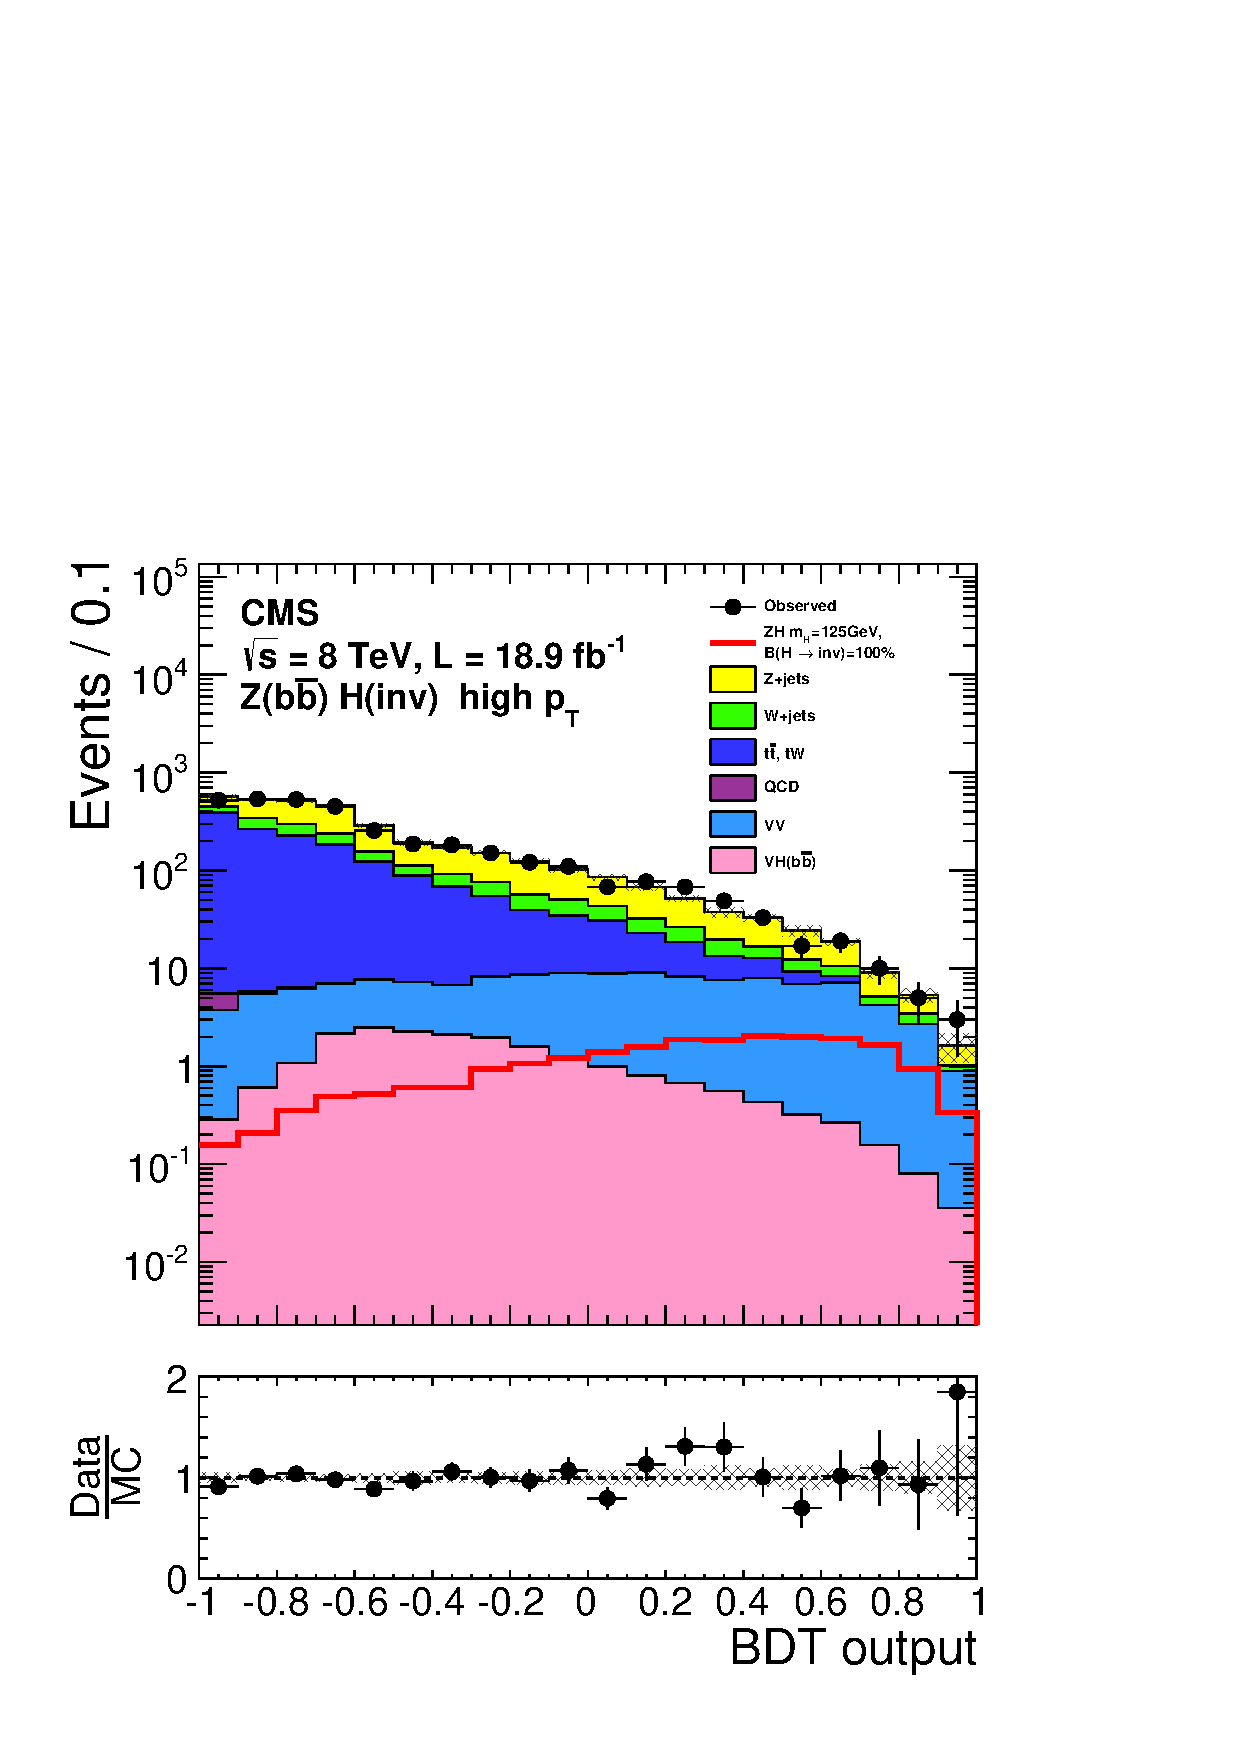
\includegraphics[clip=true,trim=0 0 20 0, width=\textwidth, height=.7\textheight]{TalkPics/panicpics/zbbbdt.pdf}
      \column{.05\textwidth}
              \hspace{-.2cm}\begin{turn}{-90}\scriptsize arXiv:1404.1344 \end{turn}
    \end{columns}
    \end{columns}

      
  \end{frame}


  \begin{frame}
    \frametitle{Combined Results}
    \begin{block}{}
      \scriptsize
      \begin{itemize}
      \item The individual limits on $\sigma$x$B(H\rightarrow inv)$ from the three channels are combined
      \item[-] SM production cross-sections are used to interpret this as a limit on B(H$\rightarrow$inv)
      \end{itemize}
    \end{block}
    \begin{columns}
      \column{.65\textwidth}
      \centering
      \begin{columns}
        \column{.95\textwidth}
      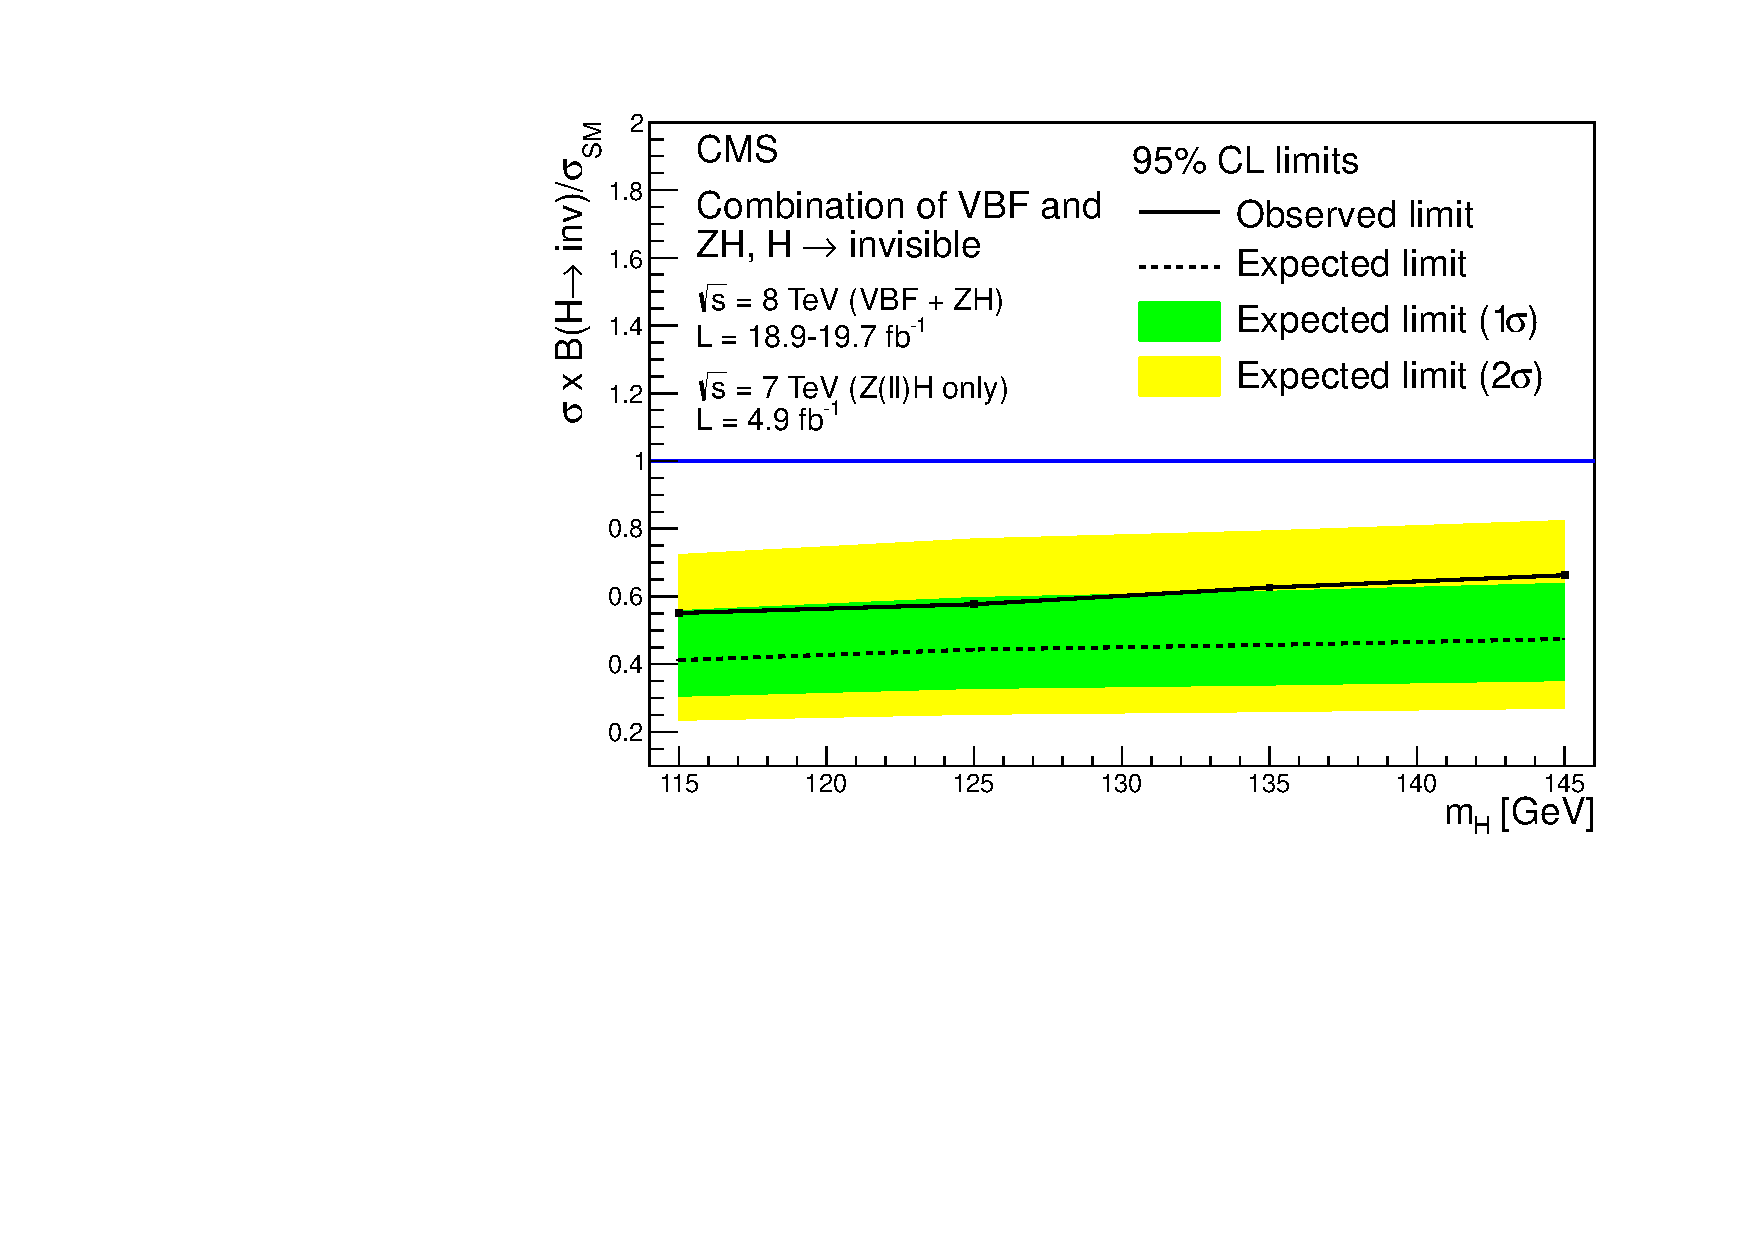
\includegraphics[clip=true,trim=0 0 0 0, width=1.1\textwidth]{TalkPics/panicpics/combinedlimit.pdf}
        \column{.05\textwidth}
        \hspace{-.4cm}\begin{turn}{-90}\scriptsize arXiv:1404.1344 \end{turn}
      \end{columns}
      \column{.35\textwidth}
      \scriptsize
      \begin{block}{}
        Observed (expected) limits on B(H$\rightarrow$inv) at 95\% C.L. for $m_{H}$=125 GeV

        \centering
        \begin{tabular}{lc}
          \hline
          Channel & Limit/\% \\
          \hline
          VBF & 65(49) \\
          ZH($\ell\ell$+bb) & 81(83) \\
          \hline
          VBF + ZH &{\color{red} 58(44)} \\
          \hline
        \end{tabular}
      \end{block}
    \end{columns}
  \end{frame}

  \begin{frame}
    \frametitle{Signatures of Dark Matter (DM)}
    \vspace{-.2cm}
    \begin{block}{}
      \scriptsize
      \begin{itemize}
      \item If DM couples to the Higgs the following diagrams are possible
      \end{itemize}
    \end{block}
    \vspace{-.2cm}
    \begin{columns}
      \column{.35\textwidth}
      \begin{block}{\scriptsize Direct Detection - e.g. LUX}
        \vspace{.3cm}
        \begin{fmfgraph*}(100,70)
          \fmfleft{i1,i2}
          \fmfright{o1,o2}
          \fmf{fermion}{i1,v1,o1}
          \fmf{fermion}{i2,v2,o2}
          \fmf{dashes,label=$H$}{v1,v2}
          \fmffreeze
          \fmflabel{$N$}{i1}
          \fmflabel{$\chi$}{i2}
          \fmflabel{$N$}{o1}
          \fmflabel{$\chi$}{o2}
        \end{fmfgraph*}
        \vspace{.3cm}
      \end{block}

      \column{.35\textwidth}
      \begin{block}{\scriptsize Invisible Higgs - LHC}
        \vspace{.3cm}
        \begin{fmfgraph*}(100,70)
          \fmfleft{i1,i2}
          \fmfright{o1,o2}
          \fmf{fermion}{i1,v1,i2}
          \fmf{fermion}{o1,v2,o2}
          \fmf{dashes,label=$H$}{v1,v2}
          \fmffreeze
          %\fmflabel{$f/w/Z$}{i1}
          \fmflabel{$\chi$}{o1}
          %\fmflabel{$f/W/Z$}{i2}
          \fmflabel{$\chi$}{o2}
        \end{fmfgraph*}
        \vspace{.3cm}
      \end{block}
      \column{.35\textwidth}
      \begin{block}{\scriptsize Annihilation - e.g. WMAP}
        \vspace{.3cm}
        \begin{fmfgraph*}(100,70)
          \fmfleft{i1,i2}
          \fmfright{o1,o2}
          \fmf{fermion}{i1,v1,i2}
          \fmf{fermion}{o1,v2,o2}
          \fmf{dashes,label=$H$}{v1,v2}
          \fmffreeze
          %\fmflabel{$f/w/Z$}{i1}
          \fmflabel{$\chi$}{i1}
          %\fmflabel{$f/W/Z$}{i2}
          \fmflabel{$\chi$}{i2}
        \end{fmfgraph*}
        \vspace{.3cm}
      \end{block}
    \end{columns}
    \begin{block}{}
      \scriptsize
      \begin{itemize}
      \item Limits on $\mathcal{B}$(H$\rightarrow$inv) therefore constrain Higgs Portal DM models
      \item[-] These constraints are directly comparable to those from other experiments
      \end{itemize}
    \end{block}
  \end{frame}

  \begin{frame}
    \frametitle{Dark Matter Interpretation - Results}
    \scriptsize
    \vspace{-.3cm}
    \begin{block}{}
      \begin{itemize}
      \item Use an effective field theory Higgs Portal model which translates B$(H\rightarrow inv)$ into a DM-nucleon cross-section (details in backup)
      \item At 90\% C.L. the CMS limit on B(H$\rightarrow$inv) is 51\% for a 125 GeV Higgs
      \item Consider three DM spin scenarios: scalar, vector, Majorana fermion:
      \item[-] CMS limits shown in green, blue and red respectively
      \end{itemize}
    \end{block}
        \vspace{-.1cm}
    \begin{columns}
      \column{1.1\textwidth}
      \begin{columns}
 
     \column{.6\textwidth}
        \hspace{1cm}\scriptsize arXiv:1404.1344
        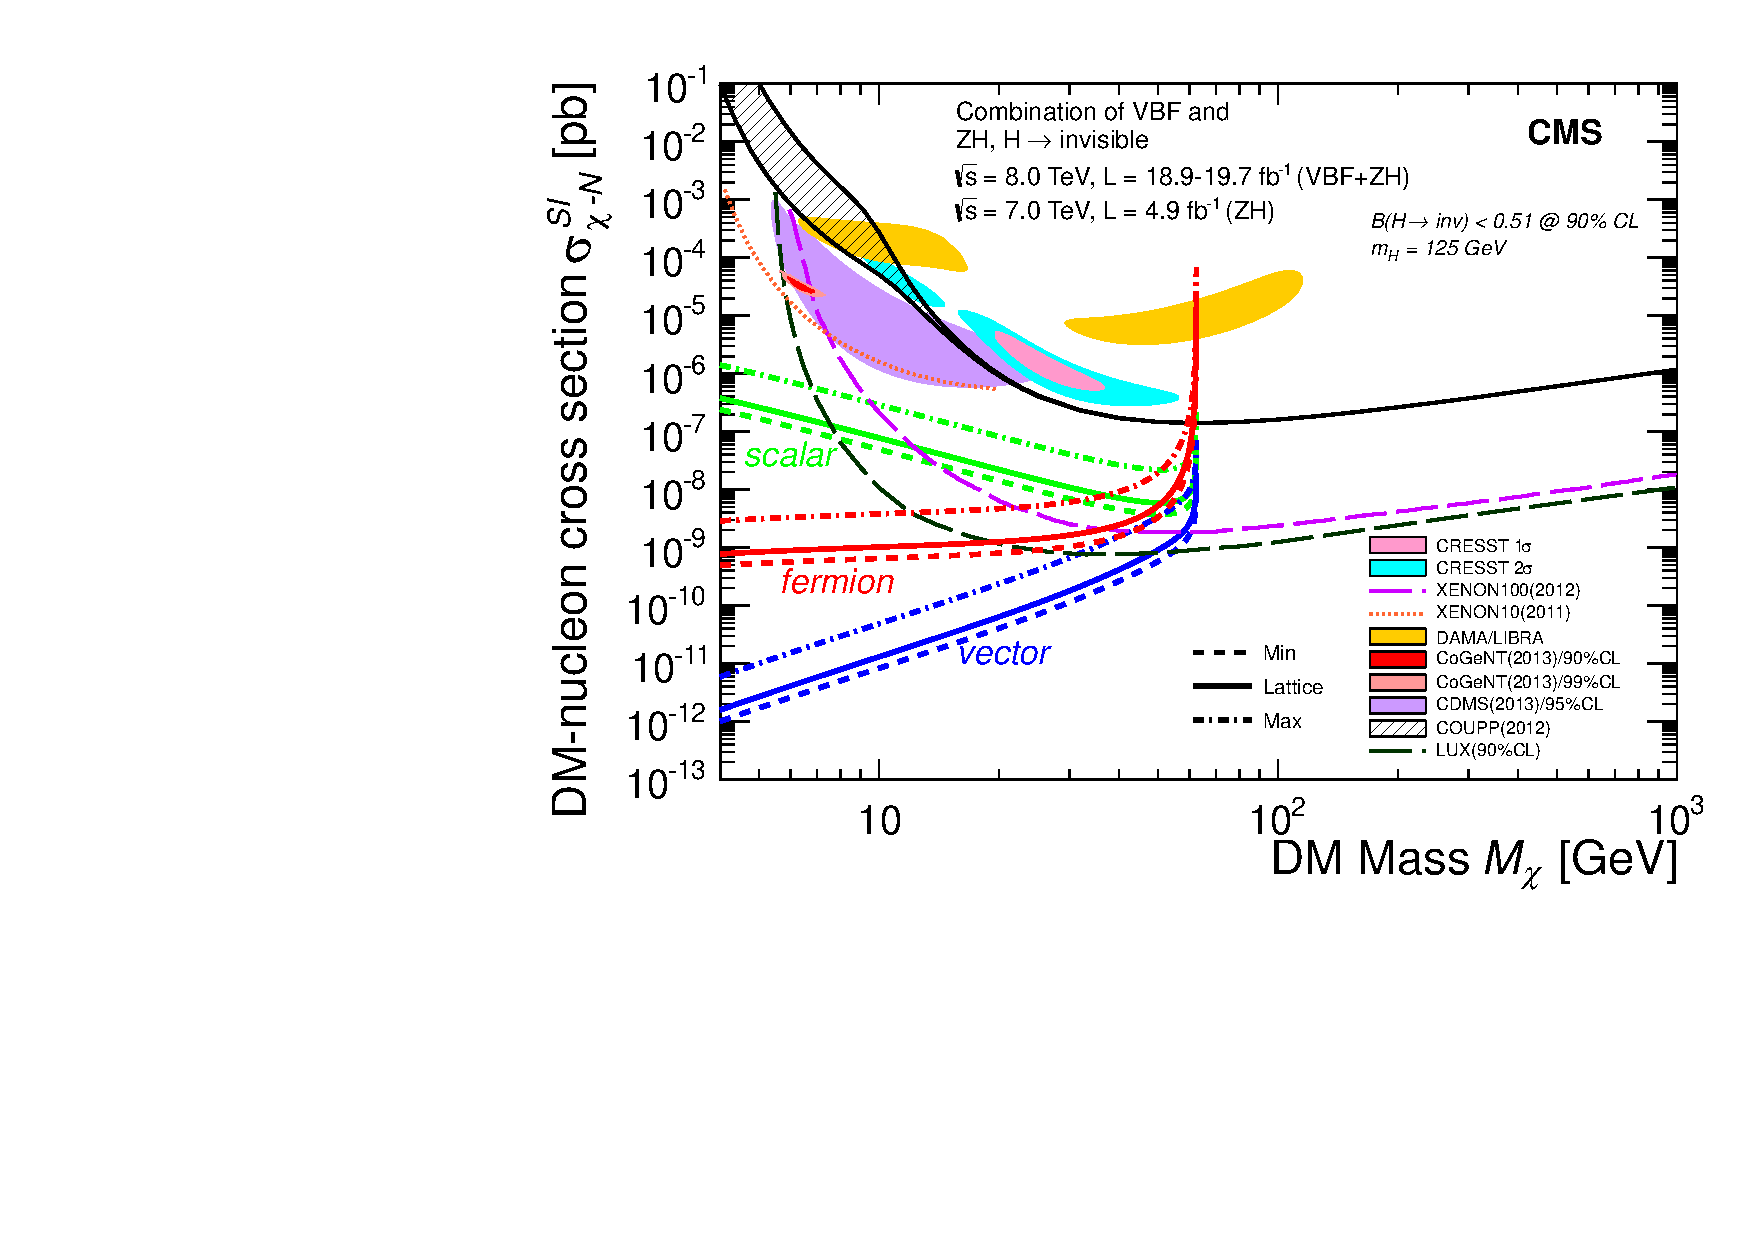
\includegraphics[clip=true,trim=0 0 0 0, height=.6\textheight, width=1.2\textwidth]{TalkPics/panicpics/dmlimit.pdf}    
        \column{.01\textwidth}
      \column{.27\textwidth}
      
      \begin{block}{}
          Min, lattice and max are varying values of Higgs-nucleon coupling

 (see backup)
          
      \end{block}

      \begin{block}{}
        $\mathcal{B}(H\rightarrow inv)$ gives important exclusion in the $M_{\chi}<m_{h}/2$ region
      \end{block}
    \end{columns}
      \end{columns}
  \end{frame}

  \begin{frame}%!!REVISIT AT END
    \frametitle{Conclusions}
    \label{lastframe}
      \begin{block}{}
        \footnotesize
        \begin{itemize}
        \item Direct searches for Higgs boson decays to invisible final sates have been carried out using the 2011 and 2012 CMS data sets:
          \vspace{-.05cm}
        \item[-] The VBF, Z($\ell\ell$)H and Z(bb)H channels have been considered
          \vspace{.05cm}
       \item[-] The mass range searched in is 105-400 GeV 
          \vspace{-.05cm}
         \item No significant excesses are seen over the background predictions
          \vspace{.05cm}
        \item The combined limit is 58(44)\% observed (expected) at 95\% C.L. for $m_{H}=125$GeV
          \vspace{-.05cm}
        \item[-] This is the most sensitive direct Higgs to invisible limit to date
        \item[-] It is broadly comparable with CMS indirect limits
          \vspace{.05cm}
        \item A Higgs portal dark matter interpretation of the above results has been presented 
          \vspace{-.05cm}
        \item[-] The results are competitive with direct DM detection experiments in the low DM mass region
        \end{itemize}
      \end{block}


  \end{frame}

  \begin{frame}%!!MAKE SURE OK
    \frametitle{References}
    \begin{block}{}
      \begin{itemize}
      \item CMS Higgs combination - CMS-PAS-HIG-14-009
      \item CMS Higgs to Invisible paper - arXiv:1404.1344
      \item CMS TWIKI with addition Higgs to Invisible results - https://twiki.cern.ch/twiki/bin/view/CMSPublic/
        Hig13030PubTWiki
      \end{itemize}
    \end{block}
  \end{frame}

  \begin{frame}
    \frametitle{Backup}
  \end{frame}


  \begin{frame}
    \frametitle{High mass combination}
    \centering
    \vspace{-.5cm}
    \begin{block}{}
      \footnotesize
      \begin{itemize}
      \item Z($\ell\ell$)H(inv) and VBF searches both go up to at least $m_{H}$=300 GeV
      \item The same combination method as used above was used to combine these two channels between 115 and 300 GeV
      \end{itemize}
    \end{block}


    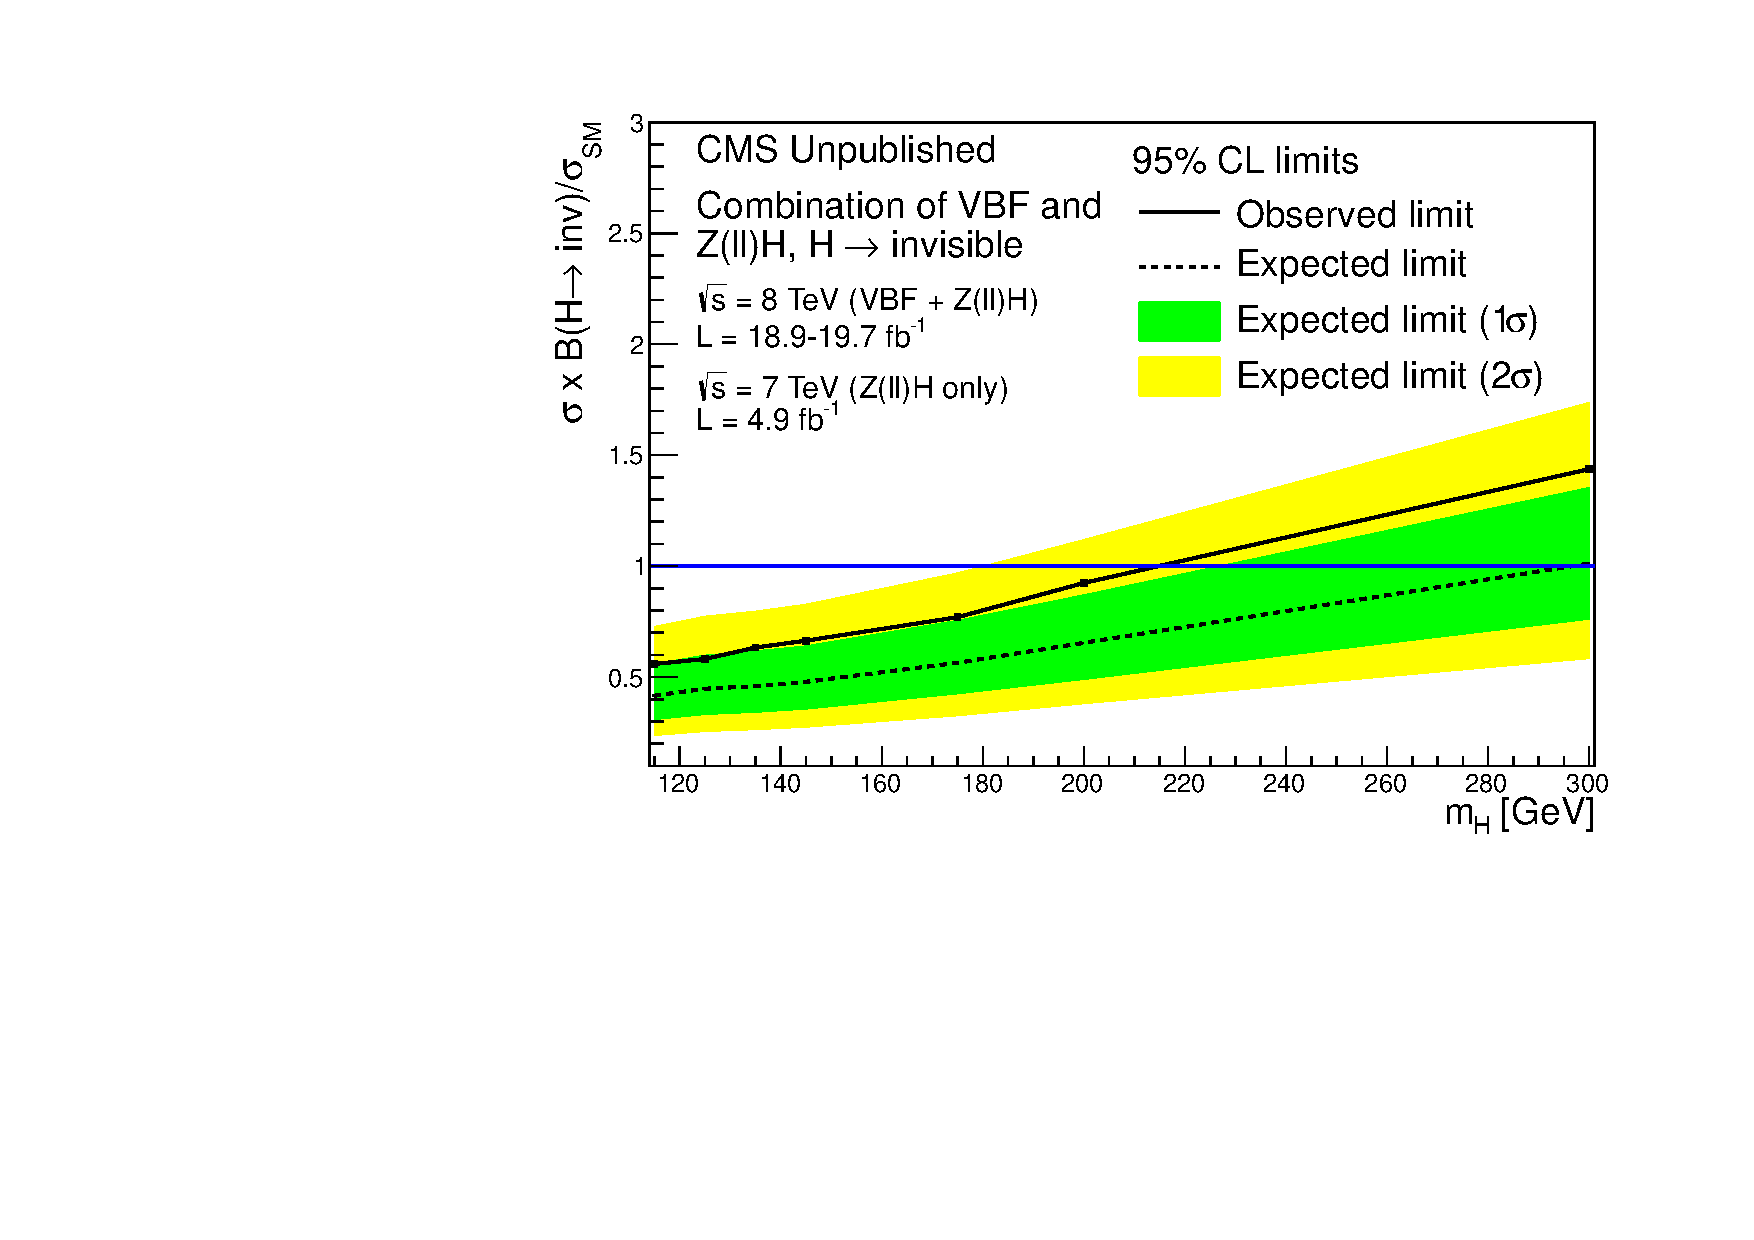
\includegraphics[clip=true,trim=0 0 0 20, width=.68\textwidth]{TalkPics/panicpics/highmasslimit.pdf}
  \end{frame}

  \begin{frame}
    \frametitle{Other direct Limits}
    \begin{block}{}
      \begin{itemize}
      \item ATLAS also produce a limit in the Z($\ell\ell$)H channel:
      \item[-] observed (expected) 75\% (62\%) at 95\% C.L.
      \end{itemize}
    \end{block}
  \end{frame}
  
  \begin{frame}
    \frametitle{DM model}
    \begin{block}{\scriptsize Formulae}
      \scriptsize
      \begin{itemize}
      \item EFT model as described in \href{http://www.sciencedirect.com/science/article/pii/S0370269312001037}{Phys.Lett. B709 (2012) 65–69}
      \item $\sigma^{SI}_{S-N} = \frac{4\Gamma_{inv}}{m_{H}^{3}v^{2}\beta}\frac{m_{N}^{4}f_{N}^{2}}{(M_{\chi}+m_{N})^{2}}$
      \item $\sigma^{SI}_{V-N} = \frac{16\Gamma_{inv}M_{\chi}^{4}}{m_{H}^{3}v^{2}\beta(m_{H}^{4}-4M_{\chi}^{2}m_{H}^{2}+12M_{\chi}^{4})}\frac{m_{N}^{4}f_{N}^{2}}{(M_{\chi}+m_{N})^{2}}$
      \item $\sigma^{SI}_{f-N} = \frac{8\Gamma_{inv}M_{\chi}^{2}}{m_{H}^{5}v^{2}\beta^{3}}\frac{m_{N}^{4}f_{N}^{2}}{(M_{\chi}+m_{N})^{2}}$
      \item[-] $m_{N}$ is the nucleon mass, 0.939 GeV
      \item[-] $f_{N}$ is the Higgs-nucleon coupling, central value 0.326, from Phys. Rev. D 81 (2010) 01453
      \item[-] Min and max values of fN from MILC collaboration Phys. Rev. Lett. 103 (2009) 122002
      \item[-] v is the Higgs vacuum expectation, 174 GeV
      \item[-] $\beta=\sqrt{1-4M_{\chi}^{2}/m_{H}^{2}}$
      \item[-] $B(H\rightarrow inv.)=\Gamma_{inv}/(\Gamma_{SM}+\Gamma_{inv})$
      \end{itemize}
    \end{block}

  \end{frame}

\end{fmffile}
\end{document}

